\documentclass[a4paper,12pt,twoside]{memoir}

% Castellano
\usepackage[spanish,es-tabla]{babel}
\selectlanguage{spanish}
\usepackage[utf8]{inputenc}
\usepackage[T1]{fontenc}
\usepackage{lmodern} % scalable font
\usepackage{microtype}
\usepackage{placeins}

\RequirePackage{booktabs}
\RequirePackage[table]{xcolor}
\RequirePackage{xtab}
\RequirePackage{multirow}

% Links
\PassOptionsToPackage{hyphens}{url}\usepackage[colorlinks]{hyperref}
\hypersetup{
	allcolors = {red}
}

% Ecuaciones
\usepackage{amsmath}

% Rutas de fichero / paquete
\newcommand{\ruta}[1]{{\sffamily #1}}

% Párrafos
\nonzeroparskip

% Huérfanas y viudas
\widowpenalty100000
\clubpenalty100000

% Evitar solapes en el header
\nouppercaseheads


\let\tmp\oddsidemargin
\let\oddsidemargin\evensidemargin
\let\evensidemargin\tmp
\reversemarginpar



% Imagenes
\usepackage{graphicx}
\newcommand{\imagen}[2]{
	\begin{figure}[!h]
		\centering
		\includegraphics[width=0.9\textwidth]{#1}
		\caption{#2}\label{fig:#1}
	\end{figure}
	\FloatBarrier
}






\graphicspath{ {./img/} }

% Capítulos
\chapterstyle{bianchi}
\newcommand{\capitulo}[2]{
	\setcounter{chapter}{#1}
	\setcounter{section}{0}
	\setcounter{figure}{0}
	\setcounter{table}{0}
	\chapter*{#2}
	\addcontentsline{toc}{chapter}{#2}
	\markboth{#2}{#2}
}

% Apéndices
\renewcommand{\appendixname}{Apéndice}
\renewcommand*\cftappendixname{\appendixname}

\newcommand{\apendice}[1]{
	%\renewcommand{\thechapter}{A}
	\chapter{#1}
}

\renewcommand*\cftappendixname{\appendixname\ }

% Formato de portada
\makeatletter
\usepackage{xcolor}
\newcommand{\tutor}[1]{\def\@tutor{#1}}
\newcommand{\tutorb}[1]{\def\@tutorb{#1}}
\newcommand{\course}[1]{\def\@course{#1}}
\definecolor{cpardoBox}{HTML}{E6E6FF}
\def\maketitle{
  \null
  \thispagestyle{empty}
  % Cabecera ----------------
\begin{center}
  \noindent
\includegraphics[width=\textwidth]{cabeceraSalud}\vspace{1.5cm}%
\end{center}
  
  % Título proyecto y escudo salud ----------------
  \begin{center}
    \begin{minipage}[c][1.5cm][c]{.20\textwidth}
        
\includegraphics[width=\textwidth]{escudoSalud.pdf}
    \end{minipage}
  \end{center}
  
  \begin{center}
    \colorbox{cpardoBox}{%
        \begin{minipage}{.8\textwidth}
          \vspace{.5cm}\Large
          \begin{center}
          \textbf{TFG del Grado en Ingeniería de la Salud}\vspace{.6cm}\\
          \textbf{\LARGE\@title{}}
          \end{center}
          \vspace{.2cm}
        \end{minipage}
    }%
  \end{center}
  
    % Datos de alumno, curso y tutores ------------------
  \begin{center}%
  {%
    \noindent\LARGE
    Presentado por \@author{}\\ 
    en Universidad de Burgos\\
    \vspace{0.5cm}
    \noindent\Large
    \@date{}\\
    \vspace{0.5cm}
    %Tutor: \@tutor{}\\ % comenta el que no corresponda
    Tutor: \@tutor{}\\
  }%
  \end{center}%
  \null
  \cleardoublepage
  }
\makeatother



% Datos de portada
\title{Aplicación web para el seguimiento de la actividad de las personas con enfermedad de Parkinson \\Documentación Técnica}
\author{Inés Martos Barbero}
\tutor{Guirguis Zaki Guirguis Abdelmessih}
\date{\today}

\begin{document}

\maketitle



\cleardoublepage



%%%%%%%%%%%%%%%%%%%%%%%%%%%%%%%%%%%%%%%%%%%%%%%%%%%%%%%%%%%%%%%%%%%%%%%%%%%%%%%%%%%%%%%%



\frontmatter


\clearpage

% Indices
\tableofcontents

\clearpage

\listoffigures

Todas las figuras en las que no se indica lo contrario, han sido elaboradas por Inés Martos Barbero, la autora de este trabajo.

\clearpage

\listoftables

Todas las tablas en las que no se indica lo contrario, han sido elaboradas por Inés Martos Barbero, la autora de este trabajo.

\clearpage

\mainmatter

\appendix




\apendice{Plan de Proyecto Software}

\section{Introducción}

bla bla bla bla bla bla bla bla bla bla bla bla bla bla bla bla bla bla bla bla bla bla bla bla bla bla bla bla bla bla bla bla bla bla bla bla bla bla bla bla bla bla bla bla bla bla bla bla bla bla bla.


\section{Planificación temporal}


\section{Planificación económica}
En una planificación económica realista hay que considerar todos los costes de realización del proyecto. Esto incluye desde la valoración económica de herramientas de desarrollo software hasta la de materiales, equipos y sueldos del personal necesario.
Además de los costos, también se debe tener en cuenta la rentabilidad a través de diversas opciones de explotación.

En este apartado se presenta la planificación económica del proyecto realizado. Se incluye el desarrollo software de la página web y el montaje hardware de un prototipo anterior sobre el que se han realizado modificaciones.

\subsection{Coste de personal}
Ha habido únicamente una persona involucrada en el proyecto, desde el desarrollo hasta el diseño, que para el cálculo de los costos de contratación será considerada Ingeniero de la Salud sin experiencia. 
En España, un Ingeniero Biomédico recién egresado o con menos de 3 años de experiencia, que es la situación que más se ajusta a este caso, puede aspirar a un salario medio bruto de 29.020 €/año \cite{jobtedIngenieroBiomedico}. Teniendo en cuenta que el contrato necesario para la realización de esté proyecto debe ser de 2 meses de duración a jornada completa, el costo del empleado será de 4.836,66 €, cantidad a la que habrá que añadirle el pago de la Seguridad Social que corre a cargo de la empresa. El cálculo de la cantidad de dinero a pagar según el Régimen General de la Seguridad Social \cite{SeguridaSocial:online} se puede calcular a través de unos porcentajes a aplicar sobre el salario bruto como se muestra en la tabla \ref{tab: costesEmpleado}.

\begin{table}[]
    \centering
    \begin{tabular}{lll}
        \hline
        \rowcolor[HTML]{FFFFFF} 
        \textbf{Sueldo bruto (€/mes)} & 2.418,33 \\ \hline
        \rowcolor[HTML]{EFEFEF} 
        \multicolumn{2}{|c|}{\textbf{Costes del Régimen General de la Seguridad Social}} \\ \hline
        \rowcolor[HTML]{FFFFFF} 
        Contingencias Comunes (23,60\%) & 570,72 \\ \hline
        \rowcolor[HTML]{EFEFEF} 
        Contrato duración determinada Tiempo Completo (6,7\%) & 162,02 \\ \hline
        \rowcolor[HTML]{FFFFFF} 
        FOGASA (0,2\%) & 4,83 \\ \hline
        \rowcolor[HTML]{EFEFEF} 
        Formación Profesional (0,6\%) & 14,51 \\ \hline
        \rowcolor[HTML]{FFFFFF} 
        \textbf{Costo total - 1 mes} & \textbf{3.170,41} \\ \hline
        \rowcolor[HTML]{C0C0C0} 
        \textbf{Costo total - 2 meses} & \textbf{6.340,82 €} \\ \hline
    \end{tabular}
    \caption{Desglose de costes de contratación}
    \label{tab: costesEmpleado}
\end{table}

\subsection{Costes de software}
Todas las herramientas software empleadas compartían la característica de ser de código abierto y gratuitas. Visual Studio Code, XAMPP, Node.js y Arduino IDE han sido algunas de las utilizadas.

\subsection{Amortización de los equipos}
El único equipo indispensable para el desarrollo del proyecto, ha sido un portátil de la marca HP (modelo HP Pavillion Laptop 15-cs2xxx) cuyo precio de compra fue de 849,45€ y al que se le estima una vida útil de 6 años. La amortización \footnote{Amortización es la pérdida de valor de un bien o activo a lo largo del tiempo.} del portatil durante los dos meses y medio que duró el trabajo puede calcularse aplicando la fórmula de la figura \ref{fig:amortizacion-portatil} , obteniendo como resultado 29,49 € \cite{Amortizacion:online}.

\begin{figure}[h]
    \centering
    \[
    \text{Amortización del Periodo} = \frac{\text{Precio de Compra}}{\text{Vida Útil en Años}} \times \frac{\text{Meses de Uso}}{12}
    \]
    \caption{Fórmula para el Cálculo de la Amortización durante un Periodo Determinado}
    \label{fig:amortizacion-portatil}
\end{figure}

\subsection{Costes de hardware}
Se va a estimar el precio del prototipo empleado para la realización de pruebas a lo largo del proyecto. En este caso el cálculo de costos se ha limitado al único dispositivo que todavía requiere mejoras pero, si se obtuviera un producto final susceptible de lanzamiento al mercado, además del cálculo del coste por unidad habría que realizar una estimación de la cantidad necesaria de cada material para la producción del número de dispositivos que se pretenda distribuir.
Tras la búsqueda y comparación de precios de todos los componentes necesarios en las tiendas online de Amazon, turiBOT y AliExpress, se opta por escoger la última de ellas ya que presenta una gran diferencia de precios \cite{AliExpre51:online}. Los resultados se pueden visualizar en la tabla \ref{tab:costesComponentes}.

\begin{table}[]
    \centering
    \begin{tabular}{ll}
        \hline
        \rowcolor[HTML]{FFFFFF} 
        \textbf{Componente} & \textbf{Coste (€)} \\ \hline
        \rowcolor[HTML]{EFEFEF} 
        Microprocesador Arduino UNO R3 & 2,00 \\ \hline
        \rowcolor[HTML]{FFFFFF} 
        Cables & 0,70 \\ \hline
        \rowcolor[HTML]{EFEFEF} 
        Acelerómetro + Giroscopio MPU-6050 & 1,17 \\ \hline
        \rowcolor[HTML]{FFFFFF} 
        Módulo bluetooth HC-05 & 4,00 \\ \hline
        \rowcolor[HTML]{EFEFEF} 
        Display LCD 16x2 & 0,71 \\ \hline
        \rowcolor[HTML]{FFFFFF} 
        Módulo I2C & 0,41 \\ \hline
        \rowcolor[HTML]{EFEFEF} 
        2 pulsadores & 0,50 \\ \hline
        \rowcolor[HTML]{FFFFFF} 
        2 resistencias & 0,50 \\ \hline
        \rowcolor[HTML]{C0C0C0} 
        \textbf{Coste Total} & \textbf{9,99 €} \\ \hline
    \end{tabular}
    \caption{Desglose de costes de los componentes}
    \label{tab:costesComponentes}
\end{table}






\section{Viabilidad legal}


\apendice{Documentación de usuario}


\section{Requisitos software y hardware para ejecutar el proyecto.}

\subsection{Software}
El desarrollo de la página web en modo localhost, en lugar de alojarla en un servidor externo, genera unos requerimientos específicos de software. Cumplir con estos requisitos es indespensable para el correcto funcionamiento de la página, asegurando el acceso a esta y permitiendo la comunicación con la base de datos y el Bluetooth del dispositivo hardware.\\

Descripción de los elementos software necesarios y sus respectivas funciones:
\begin{itemize}
    \item XAMPP. Es un paquete de software que a través de su panel de control va a permitir iniciar Apache (servidor web) y MySQL (servidor de bases de datos).
    \item Node.js. Servidor que se inicia desde los comandos de cmd y forma parte del backend para el control de la comunicación entre la web, Arduino y la base de datos.
    \item Scripts y archivos de \textit{Web\_VisualStudio}. Es imprescindible que estén localizados dentro de la carpeta htdocs de XAMPP.
    \item Visual Studio Code. Para ejecutar el archivo \textit{/bluetooth/ArduinoBridge \\ /bridge.py}, puente para la comunicación entre el dispositivo Arduino y el servidor web.
\end{itemize}

Además del software que permite el funcionamiento de la web, es indispensable cargar el script correcto en el microprocesador Arduino:
\begin{itemize}
    \item \textit{version 4.0/v4.0\_solicitudBD.ino}. Una vez el código ha sido compilado y almacenado en el microprocesador no será necesario realizar esta operación más veces, es decir, el usuario final no debería realizar este proceso ya que el hardware estaría configurado de fábrica.
    \item Arduino IDE. Necesario para realizar la subida del script.
    \item Antes de cualquier uso del prototipo hay que cargar y ejecutar el archivo MPU6050-lcd16\_ic2/MPU6050-lcd16\_ic2.ino para su calibración \cite{saragonz91:online}. Esta acción debería realizarse en fábrica, antes de la distribución al usuario final. 
\end{itemize}

Para el correcto funcionamiento de todos los softwares mencionados, se requiere la instalación de una variedad de paquetes y librerías de Arduino, python y Node.js.
\begin{itemize}
    \item Librerías de Arduino: I2Cdev, MPU6050, Wire, SoftwareSerial y LiquidCrystal\_I2C.
    \item Paquetes Pyton: PySerial, Requests.
    \item Paquetes Node.js: Express, MySQL, Body-Parser y CORS.
\end{itemize}

Se procede a la descripción detallada mediante tablas, de los requisitos funcionales específicos del proyecto software que se desarrolla. Van desde la Tabla RF-01 (Tabla \ref{RF-01}) hasta la Tabla RF-08 (Tabla \ref{RF-08}) e incluyen información del funcionamiento de la web y las interacciones con los usuarios.

\begin{table}[p]
    \centering
    \begin{tabularx}{\linewidth}{ p{0.21\columnwidth} p{0.71\columnwidth} }
        \toprule
        \textbf{RF-01}    & \textbf{Iniciar sesión}\\
        \toprule
        \textbf{Descripción}              & Todos los usuarios deben introducir de forma obligatoria su correo electrónico, tipo de usuario y contraseña para poder acceder a la página web.   \\
        \textbf{Importancia}                & Baja \\
        \bottomrule
    \end{tabularx}
    \caption{RF-01 Iniciar Sesión}
    \label{RF-01}
\end{table}

\begin{table}[p]
    \centering
    \begin{tabularx}{\linewidth}{ p{0.21\columnwidth} p{0.71\columnwidth} }
        \toprule
        \textbf{RF-02}    & \textbf{Consultar pacientes y usuarios}\\
        \toprule
        \textbf{Descripción}              & Otorgar acceso a la lista completa de usuarios o pacientes, según los permisos asignados al usuario, y permitir la realización de búsquedas específicas dentro de ella.   \\
        \textbf{Importancia}                & Media \\
        \bottomrule
    \end{tabularx}
    \caption{RF-02 Consultar pacientes y usuarios}
    \label{RF-02}
\end{table}

\begin{table}[p]
    \centering
    \begin{tabularx}{\linewidth}{ p{0.21\columnwidth} p{0.71\columnwidth} }
        \toprule
        \textbf{RF-03}    & \textbf{Gestionar pacientes y usuarios}\\
        \toprule
        \textbf{Descripción}              & Permitir la creación y eliminación de cuentas, así como la modificación de los datos almacenados en las cuentas de pacientes y médicos. La capacidad para realizar estas acciones depende del nivel de acceso que el usuario tenga en el sistema web.   \\
        \textbf{Importancia}                & Media \\
        \bottomrule
    \end{tabularx}
    \caption{RF-03 Gestionar pacientes y usuarios}
    \label{RF-03}
\end{table}

\begin{table}[p]
    \centering
    \begin{tabularx}{\linewidth}{ p{0.21\columnwidth} p{0.71\columnwidth} }
        \toprule
        \textbf{RF-04}    & \textbf{Realizar actividad}\\
        \toprule
        \textbf{Descripción}              & Ofrece las opciones de iniciar y finalizar actividades, así como la opción de guardar o descartar estas mismas.   \\
        \textbf{Importancia}                & Alta \\
        \bottomrule
    \end{tabularx}
    \caption{RF-04 Realizar actividad}
    \label{RF-04}
\end{table}

\begin{table}[p]
    \centering
    \begin{tabularx}{\linewidth}{ p{0.21\columnwidth} p{0.71\columnwidth} }
        \toprule
        \textbf{RF-05}    & \textbf{Mostrar actividades}\\
        \toprule
        \textbf{Descripción}              & Presenta al usuario en una lista las actividades realizadas por el paciente, permitiendo diferentes visualizaciones y llevar a cabo filtrados.   \\
        \textbf{Importancia}                & Alta \\
        \bottomrule
    \end{tabularx}
    \caption{RF-05 Mostrar actividades}
    \label{RF-05}
\end{table}

\begin{table}[p]
    \centering
    \begin{tabularx}{\linewidth}{ p{0.21\columnwidth} p{0.71\columnwidth} }
        \toprule
        \textbf{RF-06}    & \textbf{Consultar estadísticas}\\
        \toprule
        \textbf{Descripción}              & Visualización de los datos relacionados con las actividades realizadas por el paciente, ya sea de una actividad en concreto o de todas en conjunto.   \\
        \textbf{Importancia}                & Media \\
        \bottomrule
    \end{tabularx}
    \caption{RF-06 Consultar Estadísticas}
    \label{RF-06}
\end{table}

\begin{table}[p]
    \centering
    \begin{tabularx}{\linewidth}{ p{0.21\columnwidth} p{0.71\columnwidth} }
        \toprule
        \textbf{RF-07}    & \textbf{Gestionar cuenta}\\
        \toprule
        \textbf{Descripción}              & Facilitar a los usuarios las tareas de cambio de contraseña y actualización del correo eléctrónico vinculado a su cuenta.  \\
        \textbf{Importancia}                & Baja \\
        \bottomrule
    \end{tabularx}
    \caption{RF-07 Gestionar cuenta}
    \label{RF-07}
\end{table}

\begin{table}[p]
    \centering
    \begin{tabularx}{\linewidth}{ p{0.21\columnwidth} p{0.71\columnwidth} }
        \toprule
        \textbf{RF-08}    & \textbf{Cerrar sesión}\\
        \toprule
        \textbf{Descripción}              & Todos los usuarios tendrán la opción de cerrar sesión desde el menú de inicio. Para prevenir cierres accidentales, se solicitará una confirmación de la acción antes de que esta se complete.  \\
        \textbf{Importancia}                & Baja \\
        \bottomrule
    \end{tabularx}
    \caption{RF-08 Cerrar sesión}
    \label{RF-08}
\end{table}

\subsection{Hardware}
El funcionamiento correcto de todo el proyecto requiere del dispositivo físico adecuado que trabaje en concordancia con el software desarrollado, fin con el que se han realizado cambios y adiciones de componentes sobre el hardware del prototipo inicial. En la Tabla \ref{tab:componentes} se muestran todos los componentes empleados.

\begin{table}[]
    \begin{tabular}{|c|c|}
    \hline
    \rowcolor[HTML]{FFFFFF} 
    \multicolumn{2}{|c|}{\cellcolor[HTML]{FFFFFF}\textbf{Componentes}} \\ \hline 
    \rowcolor[HTML]{EFEFEF} 
    Arduino UNO R3 & 2 Resistencias \\ \hline
    \rowcolor[HTML]{FFFFFF} 
    Display LCD + Interfaz I2C & 2 Pulsadores \\ \hline
    \rowcolor[HTML]{EFEFEF} 
    Bluetooth HC-05 & Sensor MPU-6050 \\ \hline
    \rowcolor[HTML]{FFFFFF} 
    Cables & Caja para Prototipos \\ \hline
    \rowcolor[HTML]{EFEFEF} 
    Batería Recargable 9V + Conector de Batería & Cable Multihilo Flexible \\ \hline
    \rowcolor[HTML]{FFFFFF} 
    Proto Shield Arduino & Interruptor \\ \hline
    \rowcolor[HTML]{EFEFEF} 
    Conector 5 pines macho-hembra & \\ \hline
    \end{tabular}
    \caption{Componentes del Prototipo}
    \label{tab:componentes}
\end{table}



Los requisitos hardware se basan en el principal elemento que da pie a este proyecto, el Bluetooth, y en la necesidad de implementar mejoras para lograr una mayor facilidad de uso y comodidad. Su descripción se incluye en las tablas RF-09 ( Tabla \ref{RF-09}) a RF-12 (Tabla \ref{RF-12}).

\begin{table}[p]
    \centering
    \begin{tabularx}{\linewidth}{ p{0.21\columnwidth} p{0.71\columnwidth} }
        \toprule
        \textbf{RF-09}    & \textbf{Transmisión de datos sin cables}\\
        \toprule
        \textbf{Descripción}              & Implementación de la tecnología de comunicación escogida para que el envío de datos del dispositivo no dependa de la conexión por USB al ordenador.  \\
        \textbf{Importancia}                & Alta \\
        \bottomrule
    \end{tabularx}
    \caption{RF-09 Transmisión de datos sin cables}
    \label{RF-09}
\end{table}

\begin{table}[p]
    \centering
    \begin{tabularx}{\linewidth}{ p{0.21\columnwidth} p{0.71\columnwidth} }
        \toprule
        \textbf{RF-10}    & \textbf{Alimentación externa}\\
        \toprule
        \textbf{Descripción}              & Permitir la completa autonomía del prototipo incorporando en él una batería externa recargable. \\
        \textbf{Importancia}                & Alta \\
        \bottomrule
    \end{tabularx}
    \caption{RF-10 Alimentación externa}
    \label{RF-10}
\end{table}

\begin{table}[p]
    \centering
    \begin{tabularx}{\linewidth}{ p{0.21\columnwidth} p{0.71\columnwidth} }
        \toprule
        \textbf{RF-11}    & \textbf{Encendido y apagado del sistema}\\
        \toprule
        \textbf{Descripción}              & Regulación del flujo eléctrico que recibe el sistema. Se puede lograr de forma sencilla a través de un interruptor. \\
        \textbf{Importancia}                & Media \\
        \bottomrule
    \end{tabularx}
    \caption{RF-11 Encendido y apagado del sistema}
    \label{RF-11}
\end{table}

\begin{table}[p]
    \centering
    \begin{tabularx}{\linewidth}{ p{0.21\columnwidth} p{0.71\columnwidth} }
        \toprule
        \textbf{RF-12}    & \textbf{Seguridad y manejabilidad del prototipo}\\
        \toprule
        \textbf{Descripción}              & Es imprescindible, tanto para la protección del prototipo como para la seguridad del usuario, que el hardware y el montaje electrónico se encuentren protegidos y aislados. La solución que se implemente debe asegurar un manejo sencillo del dispositivo.  \\
        \textbf{Importancia}                & Alta \\
        \bottomrule
    \end{tabularx}
    \caption{RF-12 Seguridad y manejabilidad del prototipo}
    \label{RF-12}
\end{table}


\section{Instalación / Puesta en marcha}
Esta sección proporciona una guía detallada para que cualquier usuario pueda instalar y comenzar a utilizar el producto final de este proyecto. Se explican los procedimientos necesarios para la preparación del dispositivo y el despliegue de la web.

Antes de iniciar cualquier proceso detallado en esta sección, es imprescindible tener instalados y configurados correctamente los siguientes programas software con sus respectivas librerías y paquetes: VS Code, Node.js, XAMPP y Arduino IDE. Para más información, consultar el Anexo \textit{B.1. Requisitos software y hardware para ejecutar el proyecto} y el apartado \textit{4.2. Técnicas y herramientas} de la memoria.

\subsection{Configuración del dispositivo}
\begin{enumerate}
    \item Proceso de calibración. Abrir el archivo \textit{Arduino/version 4.0/v4.0\_soli-\\citudBD/v4.0\_solicitudBD.ino} y cargar el programa en la placa Arduino. Una vez completada la carga, se debe abrir el monitor serial, asegurándose que esté configurado para una velocidad de transmición de 115200 baudios. Para completar con éxito el proceso de calibración, el usuario debe seguir todas las instrucciones que aparecen en el monitor serial. La Figura \ref{fig:calibrado} muestra el ejemplo de un proceso de calibración adecuado, en el que los offsets presentan valores similares a la referencia.
    \begin{figure}[h]
        \centering
        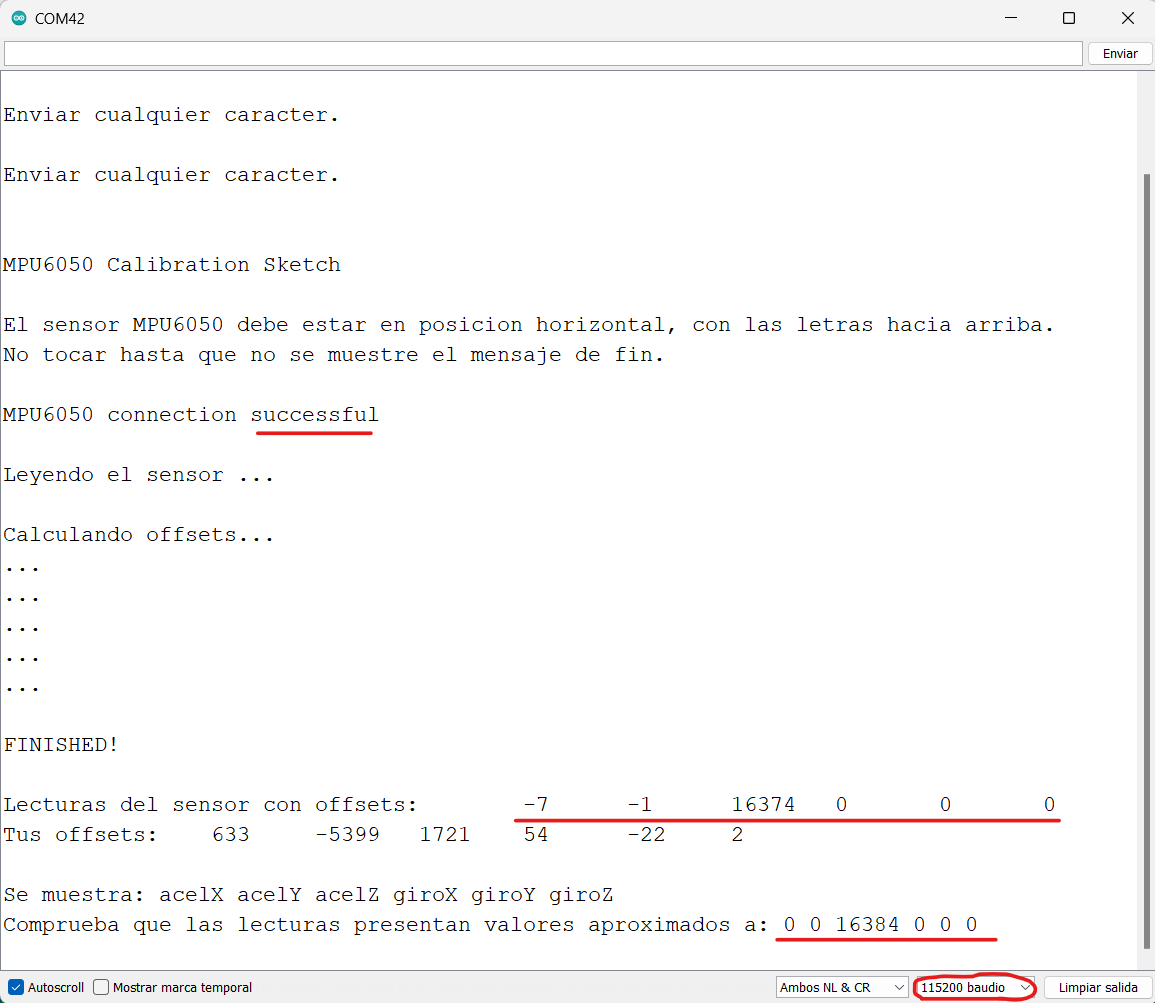
\includegraphics[width=1\textwidth]{img/B2_InstalacionPuestaMarcha/calibrado_subrayado.png}
        \caption{Proceso de calibrado.}
        \label{fig:calibrado}
    \end{figure}
    
    \item Carga del programa principal. Realizar la subida del archivo \textit{Arduino/version 4.0/v4.0\_solicitudBD/v4.0\_solicitudBD.ino} desde Arduino IDE a la placa de Arduino.
\end{enumerate}

\subsection{Despliegue de la aplicación web en entorno local}
\begin{enumerate}
    \item Acciones necesarias con XAMPP. Únicamente es necesario seguir los pasos a continuación descritos la primera vez que se descargan los archivos y se quiere desplegar la web.
    \begin{enumerate}
        \item Incluir la carpeta \textit{Web\_VisualStudio/} en el directorio \textit{xampp/htdocs} del equipo. La localización de dicho directorio puede variar según lo seleccionado durante el proceso de instalación. El repositorio de \href{https://github.com/imb1006/Web_Seguimiento_Parkinson}{GitHub} del proyecto contiene el archivo \textit{Web\_VisualStudio.zip} para facilitar la descarga.
        
        \item Iniciar Apache y MySQL desde XAMPP Control Panel (Figura \ref{fig:xampp}). Este paso sí se va a tener que realizar siempre que se quiera utilizar la plataforma web.
            \begin{figure}[h]
                \centering
                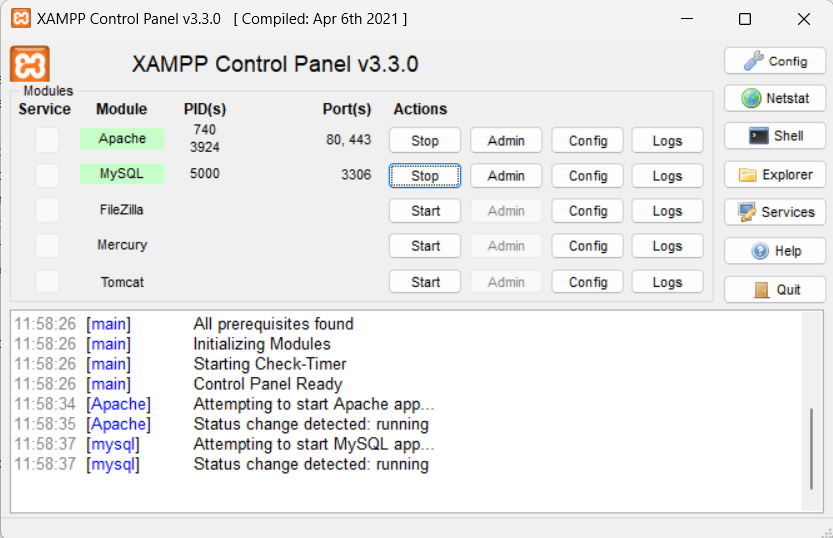
\includegraphics[width=1\textwidth]{img/B2_InstalacionPuestaMarcha/xampp.png}
                \caption{XAMPP Control Panel.}
                \label{fig:xampp}
            \end{figure}
            
        \item Crear la base de datos. Para realizar este proceso se debe navegar a la dirección \textit{localhost/phpmyadmin}, crear una nueva base de datos bajo el nombre 'WebParkinson' e importar el archivo \textit{DataBase/DataBase.sql}.
    \end{enumerate}
    
    \item Iniciar el servidor. El usuario debe dirigirse al directorio \textit{bluetooth/Ard-\\uinoServer/} y, una vez entre en él, debe abrir el terminal de comandos (cdm) haciendo clic derecho y seleccionando la opción correspondiente. Dentro del terminal, ejecutar el comando 'node server.js'. Si el proceso se realiza correctamente, aparecerá un mensaje similar al mostrado en la Figura \ref{fig:server}. En caso de que no se haya instalado MySQL en el servidor, se mostrará un mensaje de error y se deberá proceder a ejecutar el comando 'npm install mysql', tal y como se indica en la Figura \ref{fig:mysql}.

    \begin{figure}[h]
        \centering
        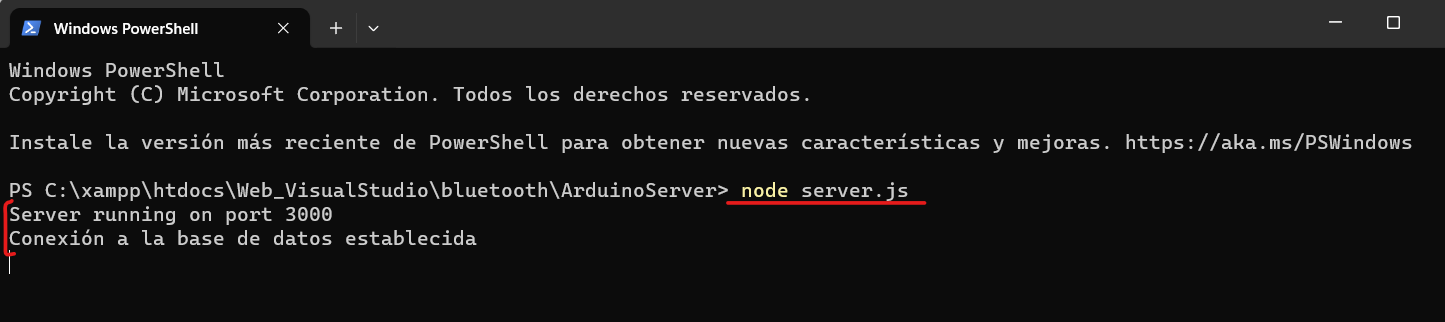
\includegraphics[width=1\textwidth]{img/B2_InstalacionPuestaMarcha/server_subrayado.png}
        \caption{Éxito en la inicialización del servidor.}
        \label{fig:server}
    \end{figure}

    \begin{figure}[h]
        \centering
        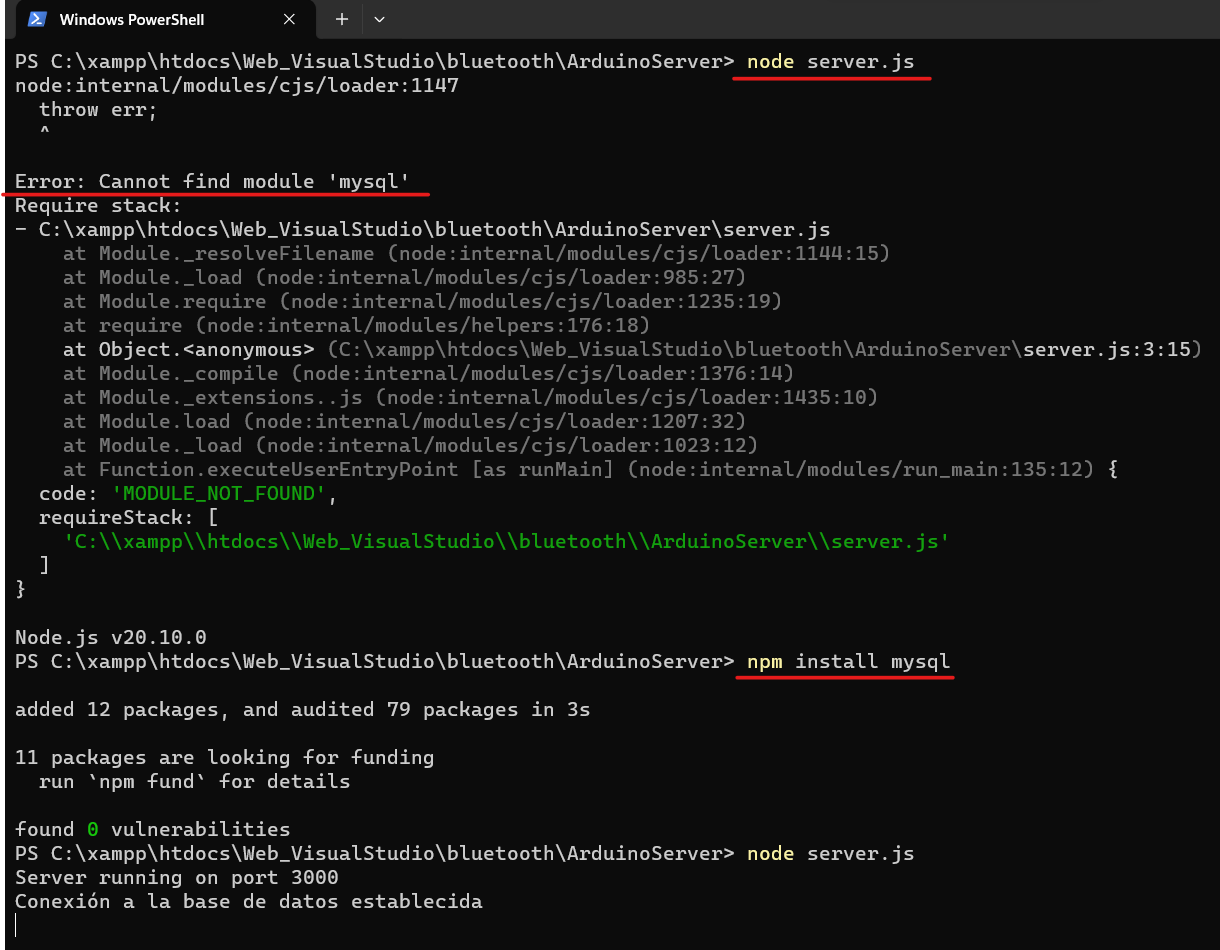
\includegraphics[width=1\textwidth]{img/B2_InstalacionPuestaMarcha/mysql_subrayado.png}
        \caption{Instalación de MySQL en el servidor.}
        \label{fig:mysql}
    \end{figure}
    
    \item Ejecutar \textit{bluetooth/ArduinoBridge/bridge.py}. La ejecución se debe realizar desde VS Code. Es importante verificar siempre el número del puerto COM asignado al Bluetooth, porque puede variar y entonces será necesario modificar el script (Figura \ref{fig:com}). En el 'Administrador de dispositivos' de Windows se puede observar el número de puerto.
    \begin{figure}[h]
        \centering
        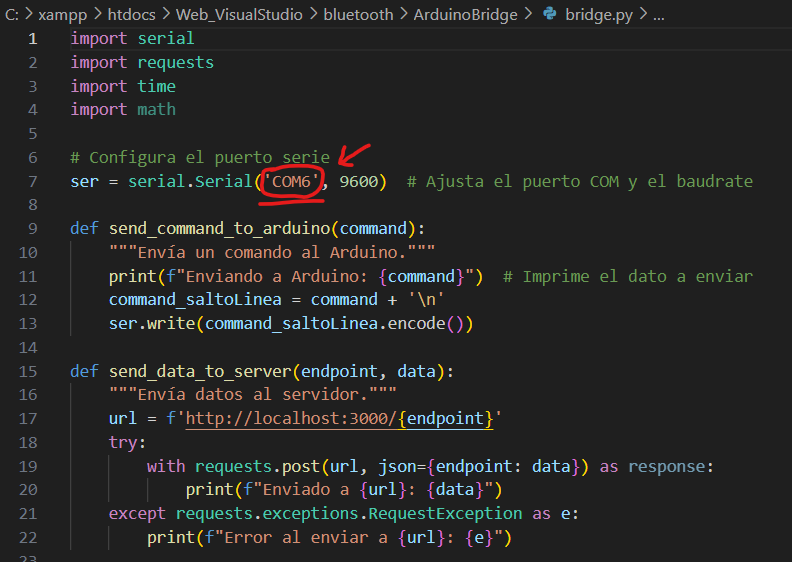
\includegraphics[width=1\textwidth]{img/B2_InstalacionPuestaMarcha/com.png}
        \caption{Fragmento del script \textit{bridge.py} en el que se debe modificar el puerto COM.}
        \label{fig:com}
    \end{figure}
    
\end{enumerate}


\section{Manuales y Demostraciones prácticas}

Para proceder a la utilización del dispositivo de monitorización de la marcha junto a la página web desarrollada, se requiere haber seguido todas las instrucciones descritas en el Anexo \textit{B.2. Instalación/Puesta en marcha}.

\subsection{Manual de uso}
Este apartado incluye las instrucciones necesarias para que cualquier persona pueda utilizar el producto desarrollado, incluso sin haber tenido contacto previo con él.

\subsubsection{Preparación}
El proceso descrito a continuación se realizará únicamente si se requiere el dispositivo de monitoreo para registrar los datos de una actividad de marcha.

\begin{enumerate}
    \item Coloque de forma correcta el dispositivo y enciéndalo. El sensor debe sujetarse mediante el velcro en el tobillo izquierdo tal y como se muestra en la Figura \ref{fig:sensor1}. La Figura \ref{fig:sensor2} permite ver cual es la posición del sensor dentro de la carcasa.
    \begin{figure}[h]
        \centering
        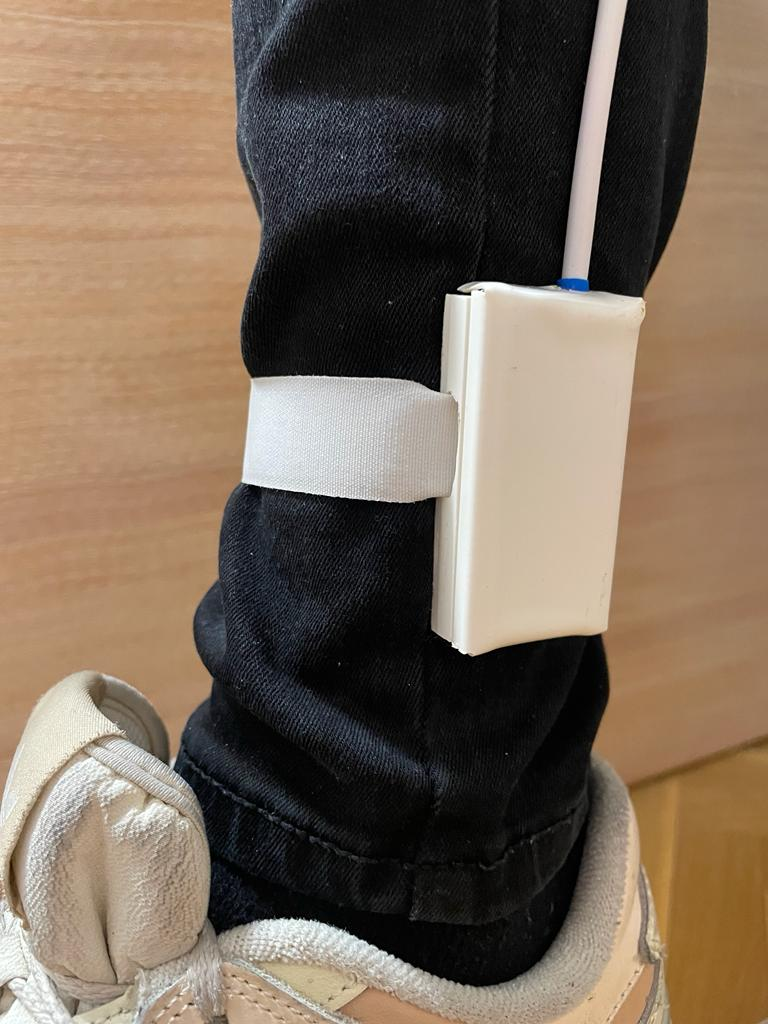
\includegraphics[width=0.3\textwidth]{img/B3_Manual/sensor1.jpg}
        \caption{Correcta colocación del sensor en el tobillo izquierdo.}
        \label{fig:sensor1}
    \end{figure}
    
    \begin{figure}[h]
        \centering
        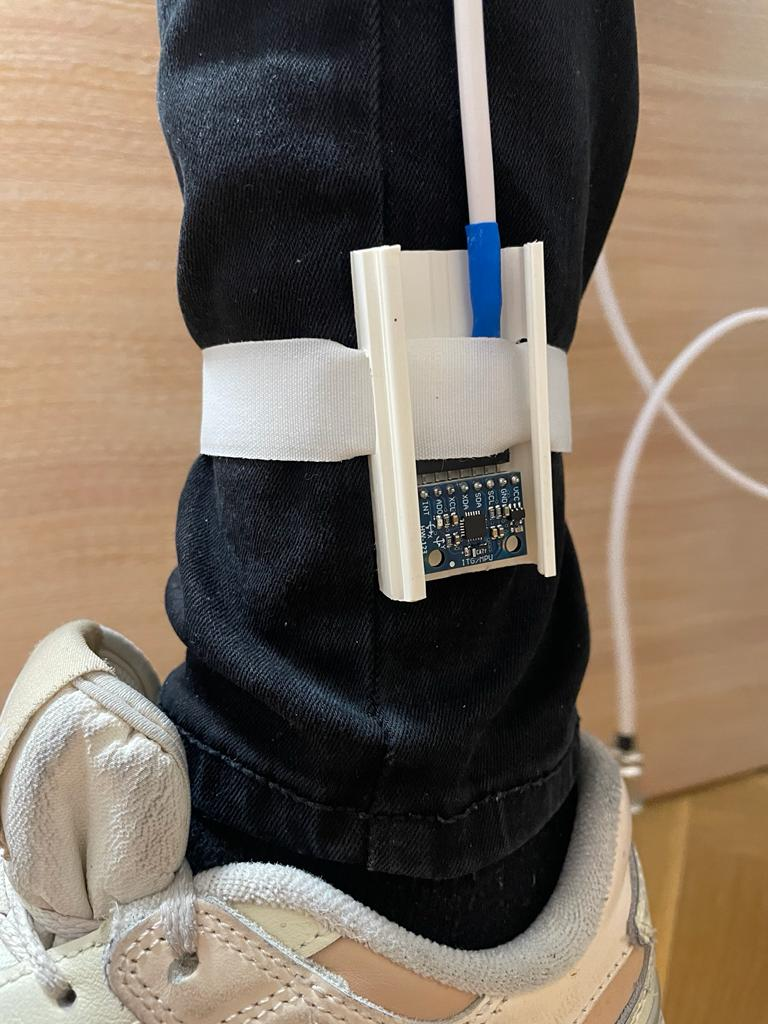
\includegraphics[width=0.3\textwidth]{img/B3_Manual/sensor2.jpg}
        \caption{Interior de la carcasa que protege al sensor MPU6050.}
        \label{fig:sensor2}
    \end{figure}
    
    \item Conexión Bluetooth desde el ordenador.
    \item Navegue a la dirección \\`\href{http://localhost/Web\_VisualStudio/common/login.html}{http://localhost/Web\_VisualStudio/common/login.html}' e inicie sesión con las credenciales de profesional o paciente.
    \item Presione el botón `Realizar Actividad' desde la ventana de visualización de la información personal del paciente. Se mostrará la pantalla de la Figura \ref{fig:RealizarActividad}, o una similar, si el usuario registrado es un paciente. Desde aquí podrá operar de forma remota y visualizar los datos de la actividad en tiempo real.
    \begin{figure}[h]
        \centering
        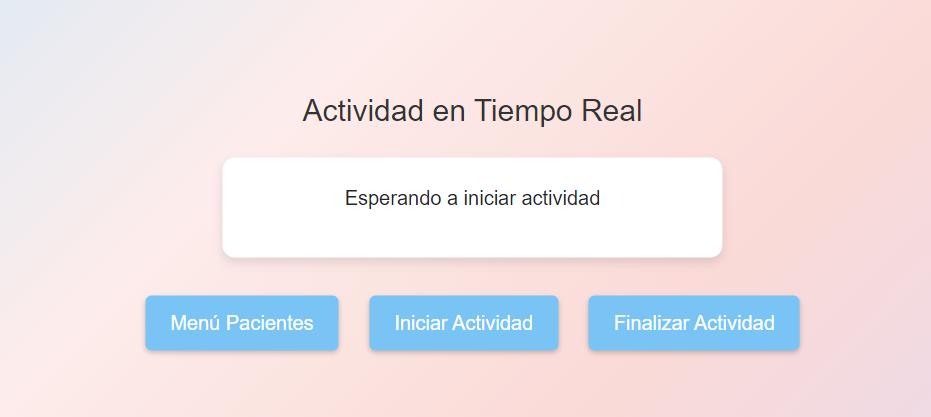
\includegraphics[width=1\textwidth]{img/B3_Manual/RealizarActividad.png}
        \caption{Pantalla para el inicio de una sesión de monitoreo.}
        \label{fig:RealizarActividad}
    \end{figure}
\end{enumerate}

\subsubsection{Utilización}
La página web ofrece distintas funcionalidades dependiendo del tipo de usuario que acceda.
Tras ir a la dirección\\ `\href{http://localhost/Web\_VisualStudio/common/login.html}{http://localhost/Web\_VisualStudio/common/login.html}' e iniciar sesión con las credenciales correspondientes, se mostrarán diferentes páginas de inicio y funcionalidades según el tipo de usuario. Las figuras \ref{fig:InicioAdmin}, \ref{fig:InicioProf} y \ref{fig:InicioPaciente} muestran capturas de pantalla de las páginas de inicio correspondientes a los usuarios de tipo administrador, profesional y paciente, respectivamente. En ellas, se pueden visualizar las principales funcionalidades para cada tipo de usuario.

\begin{figure}[h]
    \centering
    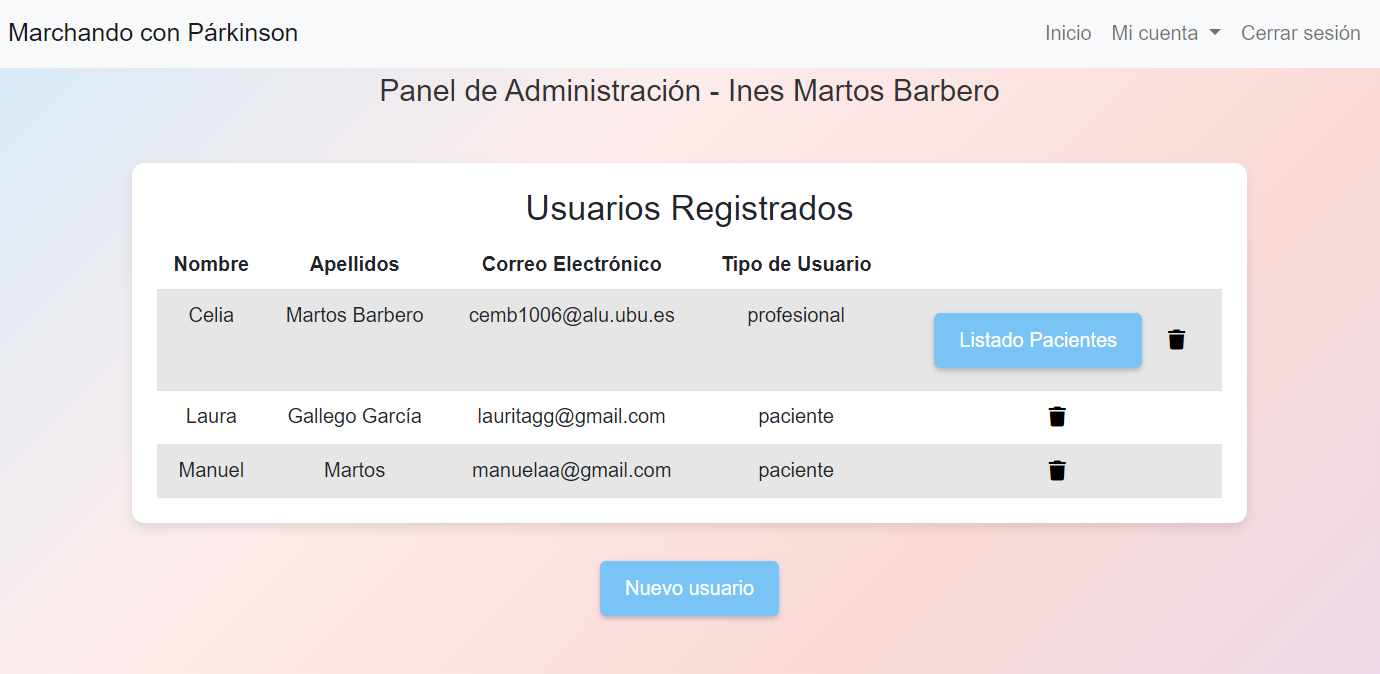
\includegraphics[width=1\textwidth]{img/B3_Manual/InicioAdmin.png}
    \caption{Pantalla de inicio para el usuario administrador.}
    \label{fig:InicioAdmin}
\end{figure}

\begin{figure}[h]
    \centering
    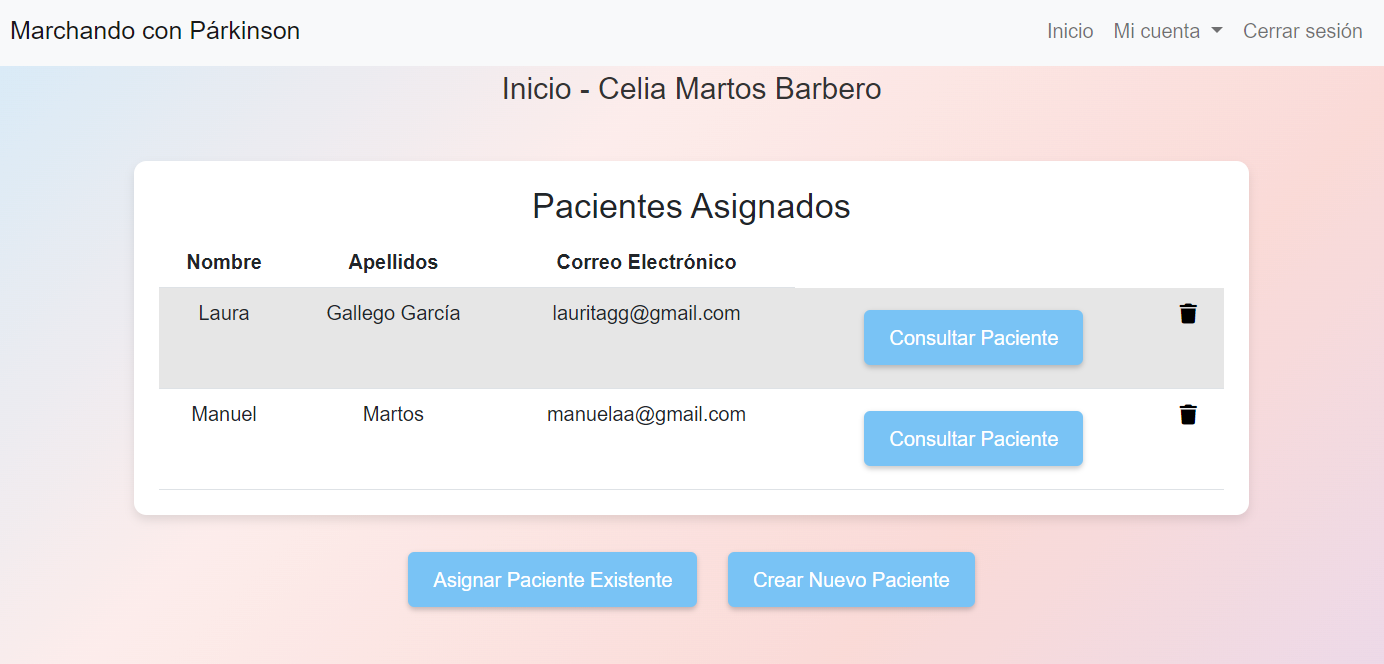
\includegraphics[width=1\textwidth]{img/B3_Manual/InicioProf.png}
    \caption{Pantalla de inicio para el usuario profesional.}
    \label{fig:InicioProf}
\end{figure}
    
\begin{figure}[h]
    \centering
    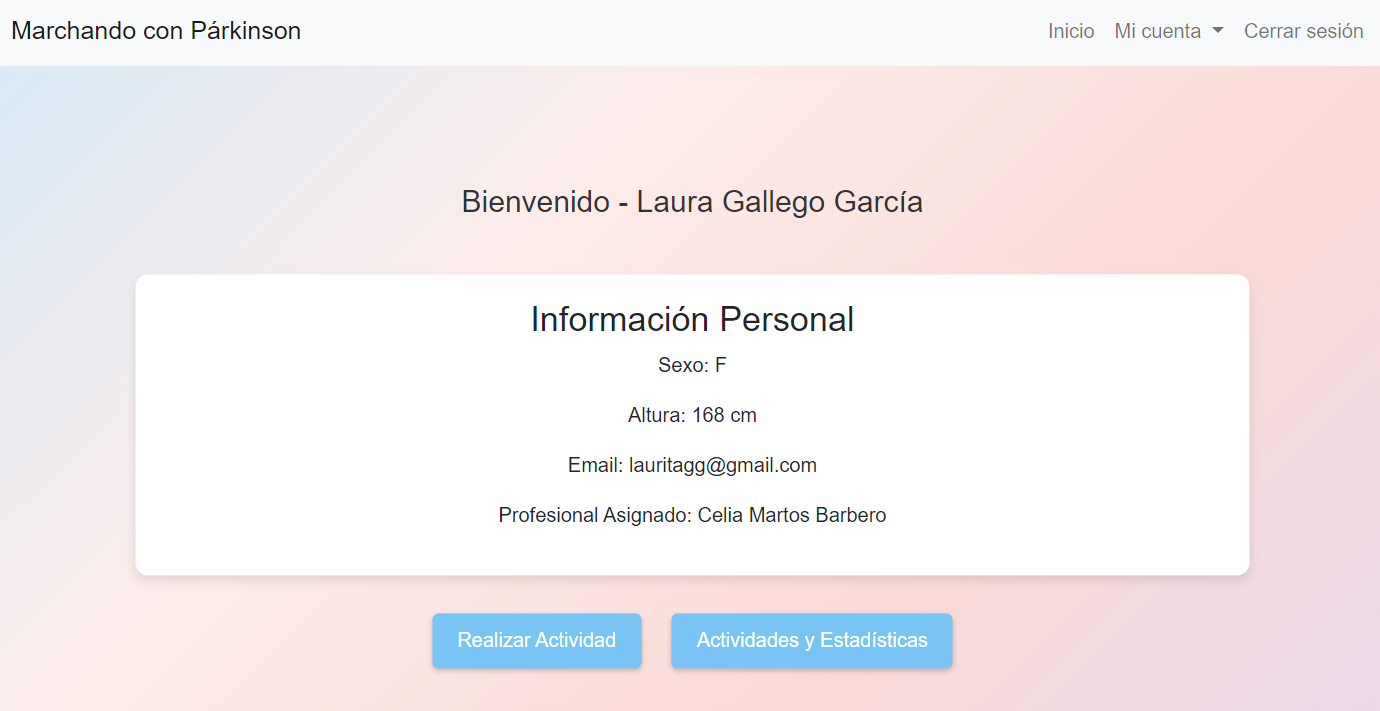
\includegraphics[width=1\textwidth]{img/B3_Manual/InicioPaciente.png}
    \caption{Pantalla de inicio para el usuario paciente.}
    \label{fig:InicioPaciente}
\end{figure}

\subsection{Demostraciones prácticas}

Vídeos explicativos:
    1) Navegación por la web.
    2) Registrar una actividad.

    
\apendice{Manual del desarrollador / programador / investigador.} % usar el término que mejor se corresponda.

\section{Estructura de directorios}

Todos los ficheros que forman parte de este trabajo se encuentran alojados en el repositorio de GitHub disponible \href{https://github.com/imb1006/Web_Seguimiento_Parkinson}{aquí}. En este apartado se detalla el contenido de cada uno de ellos para facilitar la comprensión y el análisis del trabajo.

\begin{itemize}
    \item \textbf{\textit{README.md}}.\\
    Pequeña introducción y explicación sobre el trabajo y los recursos disponibles en el repositorio de GitHub.
    \item \textbf{\textit{LICENSE}}.\\
    Documento de la licencia Apache License 2.0 utilizada para este proyecto.
    \item \textbf{\textit{Arduino/}}.\\
    Contiene todo el material, desde scripts hasta librerías, relacionado con el desarrollo del trabajo en lo relativo al software para la placa Arduino.
    \begin{itemize}
        \item \textbf{\textit{/libraries/}}.\\
        Carpeta que da acceso a algunas de librerías necesarias para el funcionamiento de los scripts de Arduino. El formato comprimido en el que se proporcionan los archivos permite su importación directa en Arduino IDE.
        \begin{itemize}
            \item \textbf{\textit{I2Cdev.zip}}
            \item \textbf{\textit{LiquidCrystal\_I2C-1.1.2.zip}}
            \item \textbf{\textit{MPU6050.zip}}
        \end{itemize}
        \item \textbf{\textit{/pruebas\_bluetooth/}}.\\
        Contiene scripts empleados al inicio del proyecto para probar de forma simple las funcionalidades de envío y recibo de datos mediante Bluetooth.
        \begin{itemize}
            \item \textbf{\textit{/01\_configuracion\_Bluetooth-HC-05/\\01\_configuracion\_Bluetooth-HC-05.ino}}: script diseñado para establecer una comunicación bidireccional entre un Arduino y un módulo Bluetooth utilizando dos pines digitales (10 y 11), en lugar de los pines de comunicación predeterminados (TX y RX). Permite comprobar de forma sencilla el funcionamiento del módulo Bluetooth a través de su conexión con un móvil para su uso con la aplicación 'Serial Bluetooth Terminal'. Además, la sencillez del script permite trabajar con el módulo Bluetooth en modo configuración (conectando pin 'EN' a 5V) y enviar comandos AT de forma eficaz.
            \item \textbf{\textit{/02\_enviar\_a\_Arduino/02\_enviar\_a\_Arduino.ino}}: permite la comunicación entre Arduino y un dispositivo Bluetooth para controlar el LED integrado en la placa mediante de comandos específicos. Se trata de un enfoque básico que sirve como prueba inicial para futuras implementaciones donde se controlarán los estados en el script de Arduino a través de botones de una página web.
            \item \textbf{\textit{/03\_recibir\_de\_Arduino/\\03\_recibir\_de\_Arduino.ino}}: establece la comunicación para el envío automático de mensajes desde el Arduino al módulo HC-05. Permite comprobar con un ejemplo básico la capacidad de envío de datos de Arduino a dispositivos Bluetooth que será necesaria en el proyecto para la transmisión de datos de actividad recogidos por el sensor MPU-6050.
            \item \textbf{\textit{/04\_envio\_recibo\_datos/\\04\_envio\_recibo\_datos.ino}}: Combina las funcionalidesdes de los dos archivos anteriores (02\_enviar\_a\_Arduino.ino y 03\_recibir\_de\_Arduino.ino).
            \item \textbf{\textit{/05\_envioBluetooth\_MPU6050/05\_envioBluetooth\\\_MPU6050.ino}}: presenta pequeños cambios para implementar la funcionalidad del envío de datos a través del módulo HC-05. Estas modificaciones se realizan sobre el script \textit{/version 2.0/MPU6050-lcd16\_ic2.ino}.
        \end{itemize}
        \item \textbf{\textit{/version 1.0/}}.\\
        Carpeta con los archivos Arduino (extensión .ino) necesarios para el funcionamiento del prototipo inicial obtenido de \cite{saragonz91:online} sin ninguna modificación.
        \begin{itemize}
            \item \textbf{\textit{/MPU6050-dmp/MPU6050-dmp.ino}}: (Extra para pruebas) activa el Digital Motion Procesor (DMP) del módulo MPU-6050. Determina y muestra el número de pasos realizados por el paciente en función de los valores pitch, roll y yaw.
            \item \textbf{\textit{/MPU6050-filtro/MPU6050-filtro.ino}}: (Extra para pruebas) script que determina la orientación del sensor utilizando unos ángulos de inclinación y rotación calculados previamente.
            \item \textbf{\textit{/MPU6050-lcd20/MPU6050-lcd20.ino}}: contiene el código para operar el prototipo usando un módulo LCD 20x4 conectado a través de un módulo I2C.
            \item \textbf{\textit{/MPU6050/MPU6050.ino}}: similar a \textit{MPU6050-lcd20.ino} pero adaptado para un LCD 16x2 y eliminando el uso del módulo I2C.
            \item \textbf{\textit{/calibracionDMP/calibracionDMP.ino}}: necesario para la calibración del DMP del módulo MPU-6050. Ajusta los offsets del acelerómetro y del giroscopio, un proceso que debe completarse en el Arduino antes de cargar el programa principal.
        \end{itemize}
        \item \textbf{\textit{/version 2.0/}}.\\
        Contiene los archivos Arduino con los que se trabajará a lo largo del proyecto, implementando funcionalidades nuevas en versiones siguientes según sea requerido.
        \begin{itemize}
            \item \textbf{\textit{/MPU6050-lcd16\_ic2/MPU6050-lcd16\_ic2.ino}}: adaptación y combinación de los scripts \\\textit{/version 1.0/MPU6050/MPU6050.ino} y \textit{/version 1.0/MPU6050-lcd20/MPU6050-lcd20.ino} para su funcionamiento con módulo LCD 16x2 e interfaz IC2.
            \item \textbf{\textit{/calibracionDMP/calibracionDMP.ino}}: no tiene modificaciones respecto al script desarrollado por \cite{saragonz91:online} y que también se encuentra en la carpeta \textit{/version 1.0/}. Este proceso de calibración del módulo MPU-6050 debe realizarse antes de su primer uso y cuando se detectan errores en las lecturas después de un uso prolongado. Tras cargar el programa en el Arduino, es en el monitor serial dónde se guía al usuario durante el proceso completo.
        \end{itemize}
        \item \textbf{\textit{/version 3.0/}}
        \begin{itemize}
            \item \textbf{\textit{/v3.0\_botonesHTML/v3.0\_botonesHTML.ino}}: proporciona al script \textit{/version 2.0/MPU6050-lcd16\_ic2/MPU6050-lcd16\_ic2.ino} la funcionalidad de controlar el inicio y detención de la medición del MPU-6050 mediante comandos recibidos por Bluetooth. Permite el control remoto del proceso de registro de datos de una actividad.
            \item \textbf{\textit{/v3.1\_mostrarDatos/v3.1\_mostrarDatos.ino}}: modifica el script proporciona al script \textit{/version 2.0/MPU6050-lcd16\_ic2/MPU6050-lcd16\_ic2.ino} para que, tanto durante la realización de la actividad como tras su finalización, los datos correspondientes sean enviados por Bluetooth.
            \item \textit{/v3.2\_ControlBotones-y-MostrarDatos/v3.2\_ControlBotones-y-MostrarDatos.ino}: combina en un solo script las funcionalidades implementadas por separado en los dos anteriores (\textit{v3.0\_botonesHTML.ino} y \textit{v3.1\_mostrarDatos.ino}). Por último, añade el número total de pasos a los datos que se envían al finalizar la actividad.
        \end{itemize}
        \item \textbf{\textit{/version 4.0/v4.0\_solicitudBD/v4.0\_solicitudBD.ino}}: es el script final del proyecto para Arduino, el que contiene la implementación de todas las funcionalidades requeridas y el que hay que cargar en la placa de Arduino UNO para el correcto funcionamiento del dispositivo en conjunto con la página web. Parte del archivo \textit{/version 3.0/v3.2\_ControlBotones-y-MostrarDatos/v3.2\_ControlBotones-y-MostrarDatos.ino}, sobre el que se realizan cambios en el código para que los datos específicos del paciente como la altura y el sexo se reciban por Bluetooth (serán obtenidos de la base de datos). 
    \end{itemize}
    \item \textbf{\textit{Documentacion\_Overleaf/}}.\\
    Carpeta que contiene todos los archivos empleados en el desarrollo de la memoria con la herramienta Overleaf. Incluye los documentos pdf de la memoria y anexos.
    \begin{itemize}
        \item \textbf{\textit{img/}}: almacena todas las imágenes que aparecen tanto en la memoria como en los anexos. Se encuentran organizadas en carpetas según su contenido y el apartado en el que han sido empleadas.
        \item \textbf{\textit{tex/}}: incluye todos los capítulos de la memoria y los anexos en sus respectivos documentos LaTeX.
    \end{itemize}
    \item \textbf{\textit{Pruebas\_Comunicación/}}.\\
    Incluye una serie de archivos y carpetas utilizados en la realización de pruebas de comunicación entre el servidor Node.js y Arduino, un proceso coordinado por el archivo \textit{bridge.py}.
    \begin{itemize}
        \item \textbf{\textit{/EnvioDatos\_a\_Arduino/}}.
        \begin{itemize}
            \item \textbf{\textit{/conNode\_html fuera/}}
        \end{itemize}
        \item \textbf{\textit{/LecturaDatos\_de\_Arduino/}}
        \begin{itemize}
            \item \textbf{\textit{/conNode\_html dentro/}}: el html que muestra los datos recibidos por Bluetooth desde Arduino, se localiza en la misma dirección que el servidor Node.js.
            \item \textbf{\textit{/conNode\_html fuera/}}: el html que muestra los datos recibidos por Bluetooth desde Arduino, se localiza en una dirección diferente a la del servidor Node.js.
            \item \textbf{\textit{/sinNode\_no funciona/}}: se intentó regular la comunicación entre la web y Arduino sin emplear un servidor Node.js pero no se logró llevar a cabo esta opción.
        \end{itemize}
    \end{itemize}
    \item \textbf{\textit{Web\_VisualStudio/}}.\\ 
    Contiene, almacenados en subcarpetas, todos los archivos y scripts de código necesarios para la creación de la página web.
    \begin{itemize}
        \item \textbf{\textit{/admin/}}.\\
        Carpeta con todos los archivos requeridos únicamente para el usuario administrador.
        \begin{itemize}
            \item \textbf{\textit{crearUsuario.php}}: procesa los datos enviados desde el formulario de \textit{crearUsuarioHTML.php}. Realiza la conexión con la base de datos y, tras una serie de validaciones, inserta la información obtenida en los campos correspondientes. Si el usuario creado es del tipo 'paciente', gestiona la asignación del profesional. Por último, establece mensajes de confirmación del proceso de creación y redirige a la página del formulario.
            \item \textbf{\textit{crearUsuarioHTML.php}}: página HTML con contenido de PHP, diseñada para mostrar el formulario de creación de usuario, cuyo diseño atractivo y responsivo se establece empleando CSS. Incluye solicitudes de validación del proceso, mensajes de retroalimentación y maneja la redirección según acciones realizadas en el proceso de creación.
            \item \textbf{\textit{eliminarUsuario.php}}: script que gestiona la eliminación de un usuario tras la confirmación al presionar el icono de papelera. Después de validar el id del usuario que se va a eliminar, se consulta su tipo en la base de datos. Según el tipo de usuario el proceso de eliminación varía: un administrador se borra únicamente de la tabla 'usuarios', un profesional requiere una reasignación de pacientes, y un paciente acarrea la eliminación de todas las actividades asociadas.
            \item \textbf{\textit{inicioAdmin.php}}: página web desarrollada con HTML, CSS y Bootstrap, diseñada para proporcionar una interfaz una interfaz para visualizar y gestionar los usuarios registrados en el sistema. Implementa la funcionalidad de confirmación de algunas operaciones. Además de consituir el front-end, interactúa con el back-end para realizar operaciones de recuperación y gestión de datos de usuarios desde la base de datos.
            \item \textbf{\textit{listadoPacientes.php}}: integra elementos de front-end y back-end para la visualización de pacientes asignados a un profesional específico. Por un lado se proporciona una interfaz de usuario con una tabla detallada de los pacientes y opciones de navegación web, y por otro se realiza la conexión con la base de datos para la obtención, procesamiento y preparación de la información de aquellos pacientes relacionados con el id del profesional que se está consultando.
            \item \textbf{\textit{menu.php}}: componente de navegación destinado a ser incluido en otras páginas web del sistema accesibles por el usuario del tipo 'administrador'. Proporciona una barra de navegación interactiva que incluye enlaces para varias funcionalidades clave: página de inicio, opciones para gestionar la cuenta del usuario y la posibilidad de cerrar sesión.
        \end{itemize}
        \item \textbf{\textit{/bluetooth/}}.
        \begin{itemize}
            \item \textbf{\textit{/ArduinoBridge/bridge.py}}: script que actúa como intermediario en la comunicación bidireccional entre Arduino y el servidor Node.js. Establece una conexión serial a través de Bluetooth con el Arduino para recibir datos y enviar comandos, utilizando la función 'send\_command\_to\_arduino(com-\\mand)'. Además, realiza solicitudes HTTP para el intercambio de información con el servidor, empleando la función 'send\_data\_to\_server(endpoint,data)'. El script mantiene una comunicación continua con una pausa mínima para evitar la sobrecarga en la transmisión de datos.
            \item \textbf{\textit{/ArduinoServer/}}.\\
            Directorio del proyecto Node.js.
            \begin{itemize}
                \item \textbf{\textit{/node\_modules/}}: carpeta que almacena todas las dependencias requeridas para el proyecto, incluye bibliotecas y frameworks instalados en Node.js.
                \item \textbf{\textit{package-lock.json}}: esencial para el bloqueo de versiones, optimización de la instalación y registro de la estructura de \textit{/node\_modules/}. Se genera de forma automática por Node Package Manager (nmp).
                \item \textbf{\textit{package.json}}: se crea de forma automática al iniciar el proceso de creación del proyecto. Contiene configuración y dependencias necesarias para el proyecto de Node.js creado.
                \item \textbf{\textit{server.js}}: archivo del servidor principal, encargado de la gestión de la aplicación web. Define rutas para solicitudes GET y POST que le permiten manejar la lógica del servidor, la interacción con la base de datos y el procesamiento de datos de entrada/salida, almacenando los datos recibidos (datos de actividades y estados de comandos) en variables esenciales para la lógica de la aplicación.
            \end{itemize}
        \end{itemize}
        \item \textbf{\textit{/common/}}\\
        Almacena una serie de archivos que implementan páginas web y funcionalidades requeridas por más de un tipo de usuario. 
        \begin{itemize}
            \item \textbf{\textit{actividad.php}}: web dinámica que permite a pacientes y profesionales monitorear y controlar actividades en tiempo real a través de botones y una interfaz sencilla de entender. Muestra información relevante de la actividad en curso (los datos que está recogiendo el sensor MPU-6050) o finalizada. Integra un script de JavaScript para manejar la interacción con el servidor y actualizar la interfaz de forma adecuada.
            \item \textbf{\textit{actualizarCorreo.php}}: maneja el proceso de actualización del correo electrónico. Tras recibir los datos del formulario, valida la información y, si es correcta, actualiza el correo del usuario en la base de datos. Si la actualización es exitosa, informa al usuario y lo redirige a la página de inicio correspondiente. En caso de errores y discrepancias, informa del problema al usuario y permanece en el formulario.
            \item \textbf{\textit{actualizarCorreoHTML.php}}: página web que proporiciona un formulario de diseño atractivo y responsivo para que el usuario actualice el correo electrónico asociado a su cuenta. Dependiendo del tipo de usuario, muestra diferentes barras de navegación. Al presionar el botón 'Aplicar Cambios', se activa la función 'confirmarAcción' de JavaScript.
            \item \textbf{\textit{cambiarContraseña.php}}: gestiona la actualización de contraseña del usuario. Comprueba que los campos del formulario se hayan rellenado y contengan la información correcta. Si los datos se verifican, procede a la actualización de la contraseña en la base de datos, informando al usuario en cada paso del proceso.
            \item \textbf{\textit{cambiarContraseña.php}}: web que presenta un formulario para que el usuario introduzca los datos requeridos para el cambio de contraseña. Al seleccionar la opción 'Aplicar Cambios', se activa la función 'confirmarAcción' de JavaScript para procesar la solicitud.
            \item \textbf{\textit{consultaActividades.php}}: proporciona, tanto a profesionales como a pacientes, una interfaz para visualizar las actividades realizadas por cada paciente y unas estadísticas básicas. Tras establecer conexión con la base de datos recupera y muestra las actividades del paciente seleccionado en una tabla detallada, llevando a cabo el cálculo de estadísticas globales como la media de bloqueos, velocidad media, número de pasos y duración media de la actividad.
            \item \textbf{\textit{eliminarCuenta.php}}: lleva a cabo la eliminación de cuentas de usuario en la web. A partir de la obtención del id del usuario que quiere eliminar su propia cuenta, procede a la eliminación llevando a cabo las operaciones requeridas según el tipo de usuario. Al finalizar se redirige al usuario al cierre de sesión (\textit{logout.php}).
            \item \textbf{\textit{login.html}}: página desarrollada como front-end para proporcionar al usuario el formulario de inicio de sesión para la web. Incluye campos para el correo eletrónico, contraseña y un desplegable para la selección del tipo de usuario. Utiliza estilos personalizos y emplea herramientas como HTML, CSS y JavaScript.
            \item \textbf{\textit{login.php}}: manejo, desde el back-end, del proceso de inicio de sesión. Realiza la autenticación de las credenciales introducidas en el formulario de inicio de sesión. Si los datos resultan correctos, almacena la información del usuario en la sesión y lo redirige a la página de inicio correspondiente según su rol.
            \item \textbf{\textit{logout.php}}: control del proceso de cierre de sesión en la web. Al confirmar el usuario que quiere cerrar sesión se va a ejecutar este script para iniciar la sesión activa, eliminar todas las variables de sesión y destruir la sesión. Finalmente, redirige al usuario a la página de inicio de sesión (\textit{login.html}).
        \end{itemize}
        \item \textbf{\textit{/database/DataBase.sql}}: script de SQL para la creación y configuración de la base de datos 'webparkinson', facilitando su importación a phpMyAdmin. Se encarga de estructurar las tablas 'actividades', 'pacientes', 'profesional\_paciente' y 'usuarios', definiendo para cada una campos específicos, tipos de datos y restricciones. Se establecen claves primarias para identificación única y claves extranjeras para definir relaciones entre tablas. Además, se incluye la inserción de datos en la tabla usuarios, creando un usuario administrador y un usuario profesional, imprescindible para el uso inicial de la web.
        \item \textbf{\textit{/js/confirmacion.js}}: archivo de JavaScript que proporciona métodos de confirmación y redirección para diversas acciones críticas de la página web. Este script contiene tres funciones princiaples: \textit{'realizarRedireccion(userType)'}, que redirige al usuario a la página de inicio correspondiente según su tipo (administrador, profesional o paciente), \textit{'confirmarAccion(accion)'}, que muestra mensajes de confirmación para distintas acciones; y \textit{'confirmarAccionConId(accion,id)'}, que es similar a la anterior pero se utiliza para acciones que requieren un identificador específico. Estas funciones mejoran la interactividad y la seguridad de la aplicación web.
        \item \textbf{\textit{/paciente/}}\\
        Contiene scripts que serán únicamente empleados por usuarios de tipo paciente.
        \begin{itemize}
            \item \textbf{\textit{inicioPaciente.php}}: página de inicio para pacientes que muestra su información personal y opciones para iniciar actividad o consultar estadísticas anteriores. Mediante JavaScript interacciona con Arduino para proporcionar datos de altura y sexo.
            \item \textbf{\textit{menu.php}}: componente de navegación destinado a ser incluido en otras páginas web del sistema accesibles por el usuario del tipo 'paciente'. Proporciona una barra de navegación interactiva que incluye enlaces para varias funcionalidades clave: página de inicio, opciones para gestionar la cuenta del usuario y la posibilidad de cerrar sesión.
        \end{itemize}
        \item \textbf{\textit{/profesional/}}\\
        Carpeta que contiene los scripts con funcionalidades y características exclusivas del usuario de tipo profesional.
        \begin{itemize}
            \item \textbf{\textit{asignarPaciente.php}}: script que maneja la asignación de pacientes al profesional actualmente en sesión. En primer lugar recibe el id del paciente y tras su validación ejecuta la consulta SQL para realizar la asignación solicitada. Tras finalizar el proceso se proporciona un mensaje de confirmación.
            \item \textbf{\textit{infoPaciente.php}}: página web que muestra la información detallada de un paciente específico mediante el empleo de una cookie que recoge el id del paciente. Realiza una conexión con la página web para obtener toda la información requerida y através de JavaScript envía a Arduino datos los datos obtenidos de altura y sexo necesarios si se quiere iniciar una actividad. También presenta diferentes botones que redirigen a otras funcionalidades.
            \item \textbf{\textit{inicioProfesional.php}}: página de inicio para profesionales diseñada para mostrar la lista de pacientes asignados junto a funcionalidades para la consulta de información detallada, así como opciones para asignar nuevos pacientes o eliminar existentes. Se utiliza Bootstrap y CSS para un diseño claro y accesible.
            \item \textbf{\textit{menu.php}}: componente de navegación destinado a ser incluido en otras páginas web del sistema accesibles por el usuario del tipo 'profesional'. Proporciona una barra de navegación interactiva que incluye enlaces para varias funcionalidades clave: página de inicio, opciones para gestionar la cuenta del usuario y la posibilidad de cerrar sesión.
            \item \textbf{\textit{mostrarPacientes.php}}: web que permite a los profesionales visualizar una tabla de pacientes que no les pertenecen y la posibilidad de asignarselos a través de un botón interactivo que redirige a \textit{asignarPaciente.php}.
            \item \textbf{\textit{nuevoPaciente.php}}: gestión del proceso de creación de nuevos pacientes. Incluye validaciones de los datos introducidos en cada campo, tras las cuales inserta al nuevo paciente en la base de datos y lo asigna al profesional cuyo id se ha almacenado. La finalización exitosa del proceso se confirma a través de una ventana emergente.
            \item \textbf{\textit{nuevoPacienteHTML.php}}: página web que proporciona un formulario con un diseño responsivo para incresar los datos del nuevo paciente. Se almacena el id del profesional para que la asignación posterior se realice de forma correcta. Presenta una serie de botones que permiten cancelar o continuar con la operación en cualquier momento.
            \item \textbf{\textit{quitarPaciente.php}}: script de php que, tras verificar la conexión con la base de datos y el id del paciente a eliminar, elimina la relación con el profesional de la tabla 'profesional\_paciente'. Además, si dicho paciente no se encuentra asignado a otros profesionales, se llevan a cabo los siguientes pasos: eliminar actividades asociadas al paciente, eliminar el registro de la tabla 'pacientes' y, eliminar el registro de la tabla 'usuarios'. Si la acción se lleva a cabo con éxito, se notifica al usuario profesional.
        \end{itemize}
    \end{itemize}
\end{itemize}


\section{Compilación, instalación y ejecución del proyecto}

En caso de ser necesaria esta sección, porque la compilación o ejecución no sea directa.


\section{Pruebas del sistema}
Esta sección puede ser opcional.

Puede tratarse de validación de la interfaz por parte de los usuarios, mediante escuestas o similar o validación del funcionamiento mediante pruebas unitarias.



\section{Instrucciones para la modificación o mejora del proyecto.}

Instrucciones y consejos para que el trabajo pueda ser mejorado en futuras ediciones.
\apendice{Descripción de adquisición y tratamiento de datos}


\section{Descripción formal de los datos}

Tablas, imágenes, señales, secuencias de ADN…
    
\section{Descripción clínica de los datos.}

Descripción y explicaciones clinicas del significado o interpretación de los datos.
\apendice{Manual de especificación de diseño}

\section{Planos}
El montaje inicial, del que parte la idea de este proyecto con el objetivo principal de desarrollar un dispositivo completamente autónomo, se presenta en la Figura \ref{fig:arqInicio}.

\begin{figure}[h]
    \centering
    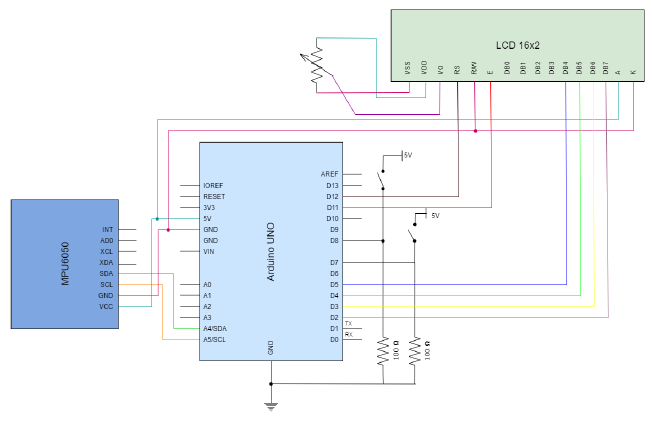
\includegraphics[width=1\textwidth]{img/E1_Planos/planoSara.png}
    \caption{Esquema de montaje del prototipo de partida. \cite{saragonz91:online}}
    \label{fig:arqInicio}
\end{figure}

Durante el trabajo se ha implementado una fuente de alimentación externa, regulada a través de un interruptor, y un módulo Bluetooth destinado a la transmisión de datos. La instalación del módulo HC-05 requiere únicamente cuatro conexiones: conectar Vcc al polo positivo, GND a toma de tierra, y las conexiones TXD (pin de transmisión) y RXD (pin de recepción) a los correspondientes opuestos en la placa Arduino, que en este caso se han configurado como los pines digitales 10 (RX) y 11 (TX). El montaje final se refleja en la Figura \ref{fig:arqFinal}.

\begin{figure}[h]
    \centering
    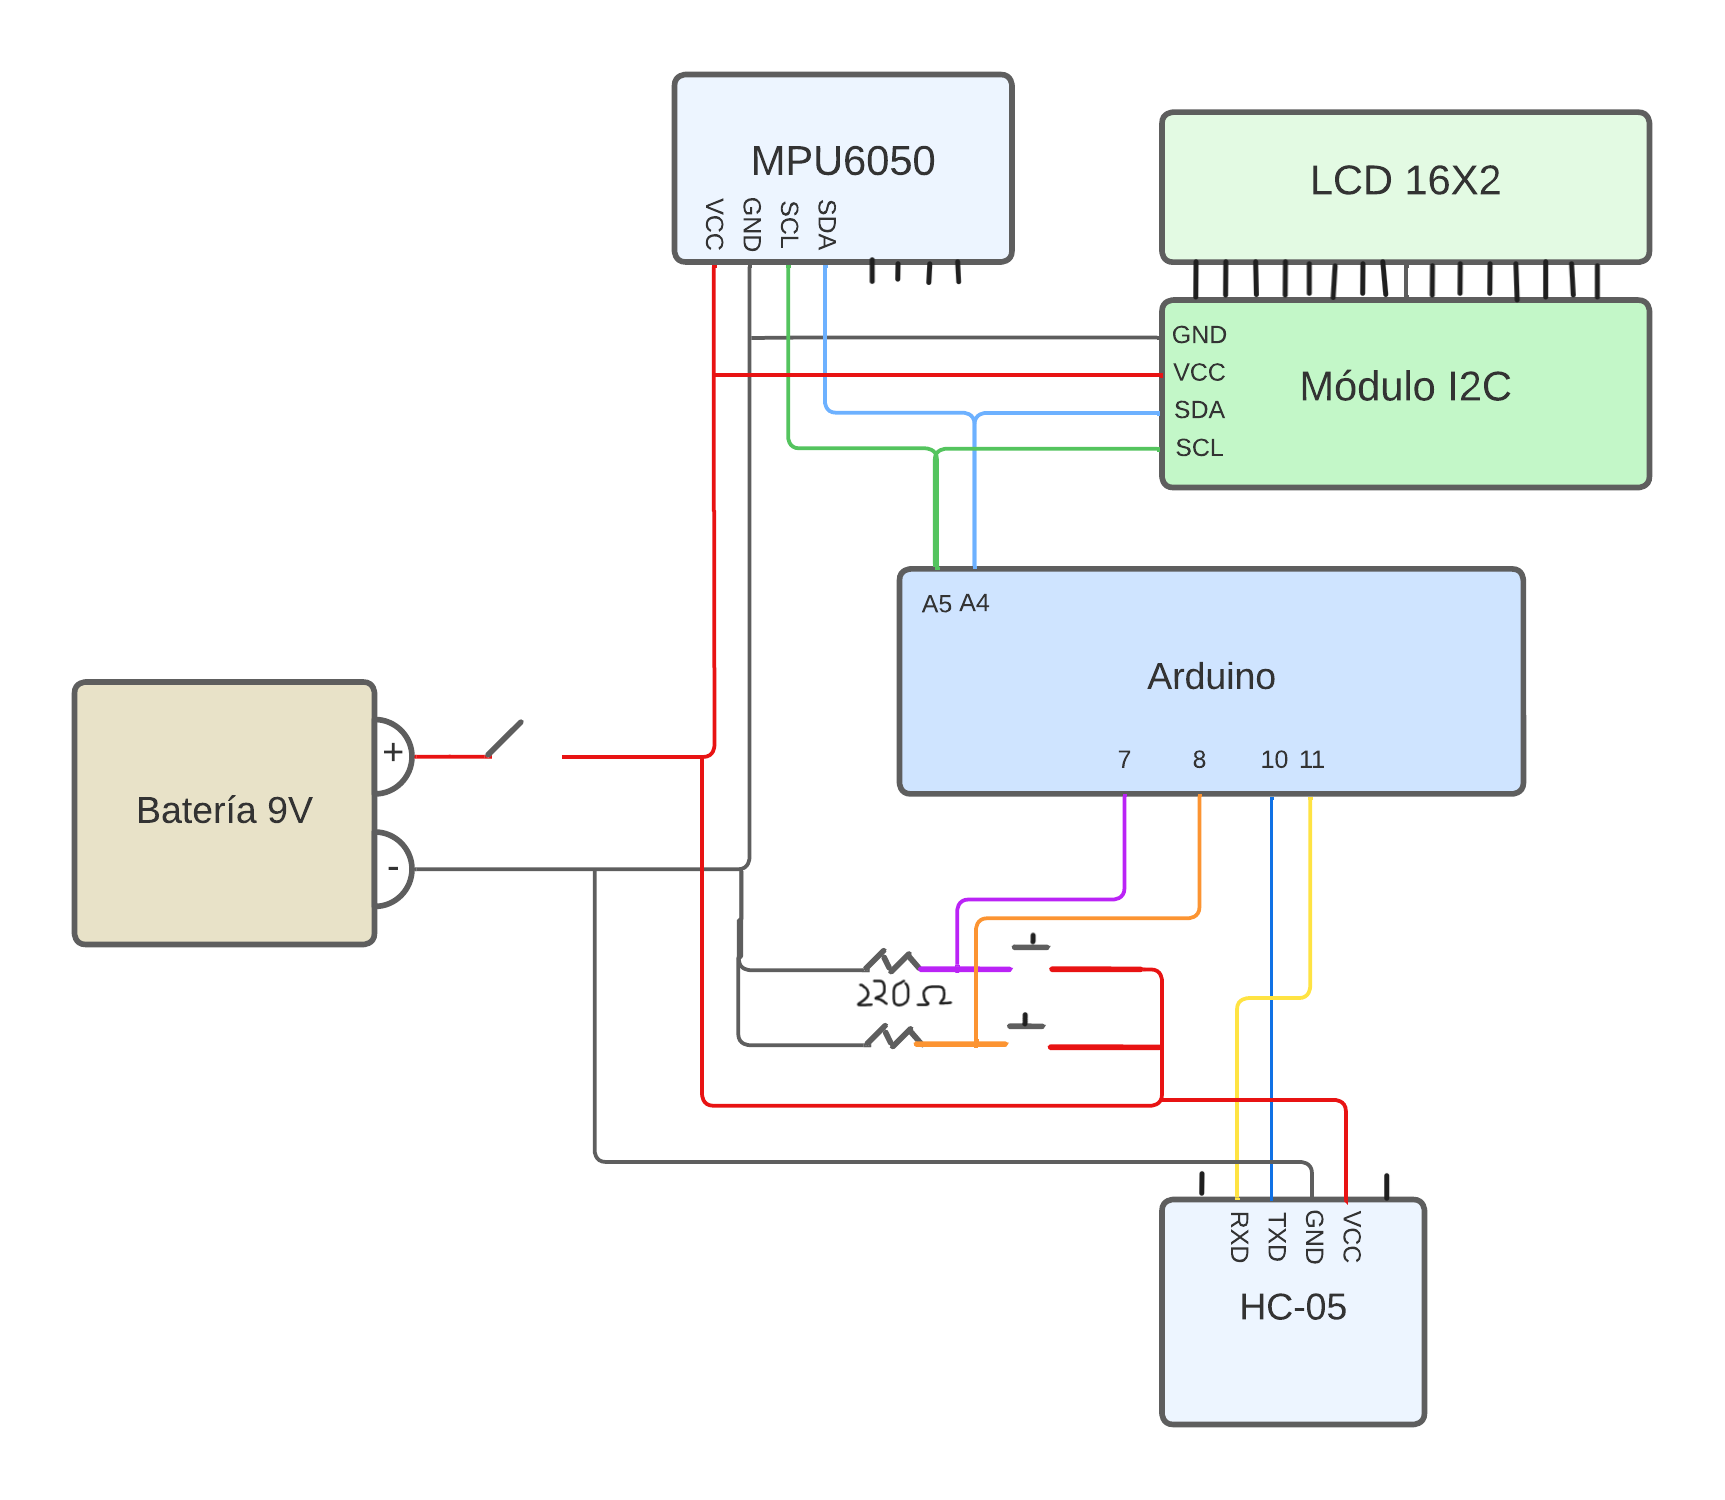
\includegraphics[width=1\textwidth]{img/E1_Planos/EsquemaArduino.png}
    \caption{Esquema de montaje del dispositivo final.}
    \label{fig:arqFinal}
\end{figure}

El protipo final, ilustrado en la Figura \ref{fig:hardwareFinal}, integra todos los componentes de hardware esenciales para facilitar su manejo.

\begin{figure}[h]
    \centering
    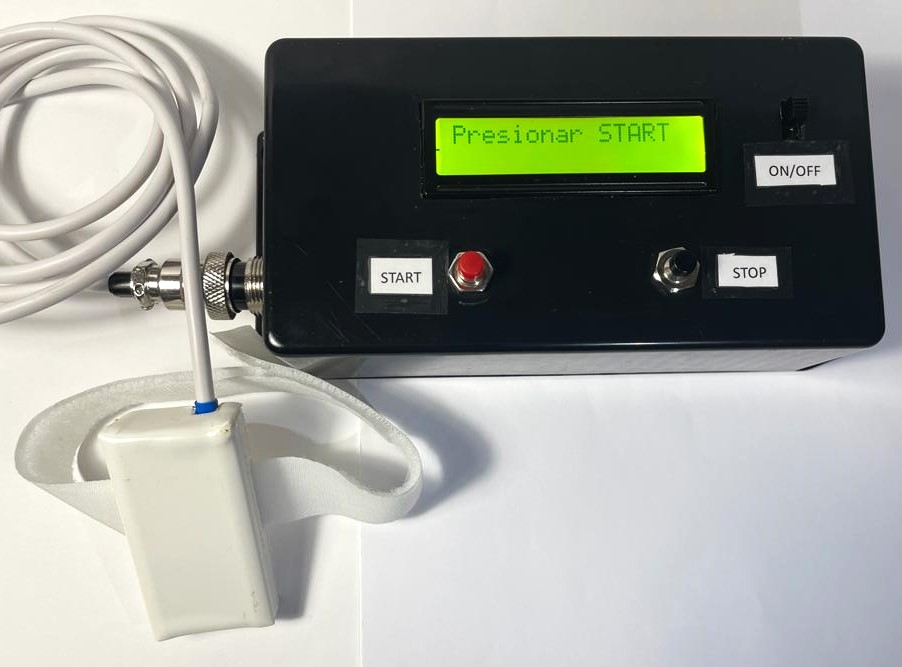
\includegraphics[width=0.7\textwidth]{img/E1_Planos/montajeFinal.jpg}
    \caption{Hardware del dispositivo final.}
    \label{fig:hardwareFinal}
\end{figure}


\section{Diseño arquitectónico}
El diseño de la arquitectura web es el primer paso crítico en el diseño de software. Partiendo de los requisitos del sistema, el diseño arquitectónico proporciona una planificación y organización global de este, establenciendo las relaciones entre sus componentes \cite{castro2015arquitectura}.

Este proceso inicia con la obtención de los requisitos funcionales, detallados en el \textit{Anexo B.1}. Sin embargo, el paso esencial para la arquitectura web es el diseño de la experiencia de usuario. En este caso, se emplean diagramas de flujo que muestran las posibilidades del sistema para cada tipo de usuario.

Descripción del diagrama de flujo:
\begin{itemize}
    \item Figura \ref{fig:0_InicioFin}. Muestra el proceso de iniciar sesión en la página web y las opciones que comparten los usuarios en el menú. Redirige a otras figuras diferentes donde el diagrama de flujo continúa según el tipo de usuario que haya iniciado sesión.
    \item Figura \ref{fig:1_Admin}. Recorre las opciones presentadas al administrador en el sistema.
    \item Figura \ref{fig:2_Profesional}. Presenta el flujo de funcionalidades accesibles para el profesional y la relación entre ellas.
    \item Figura \ref{fig:3_Paciente}. Indica la forma de navegación del paciente en la web y la forma de acceder a cada acción posible.
\end{itemize}


\begin{figure}[h]
    \centering
    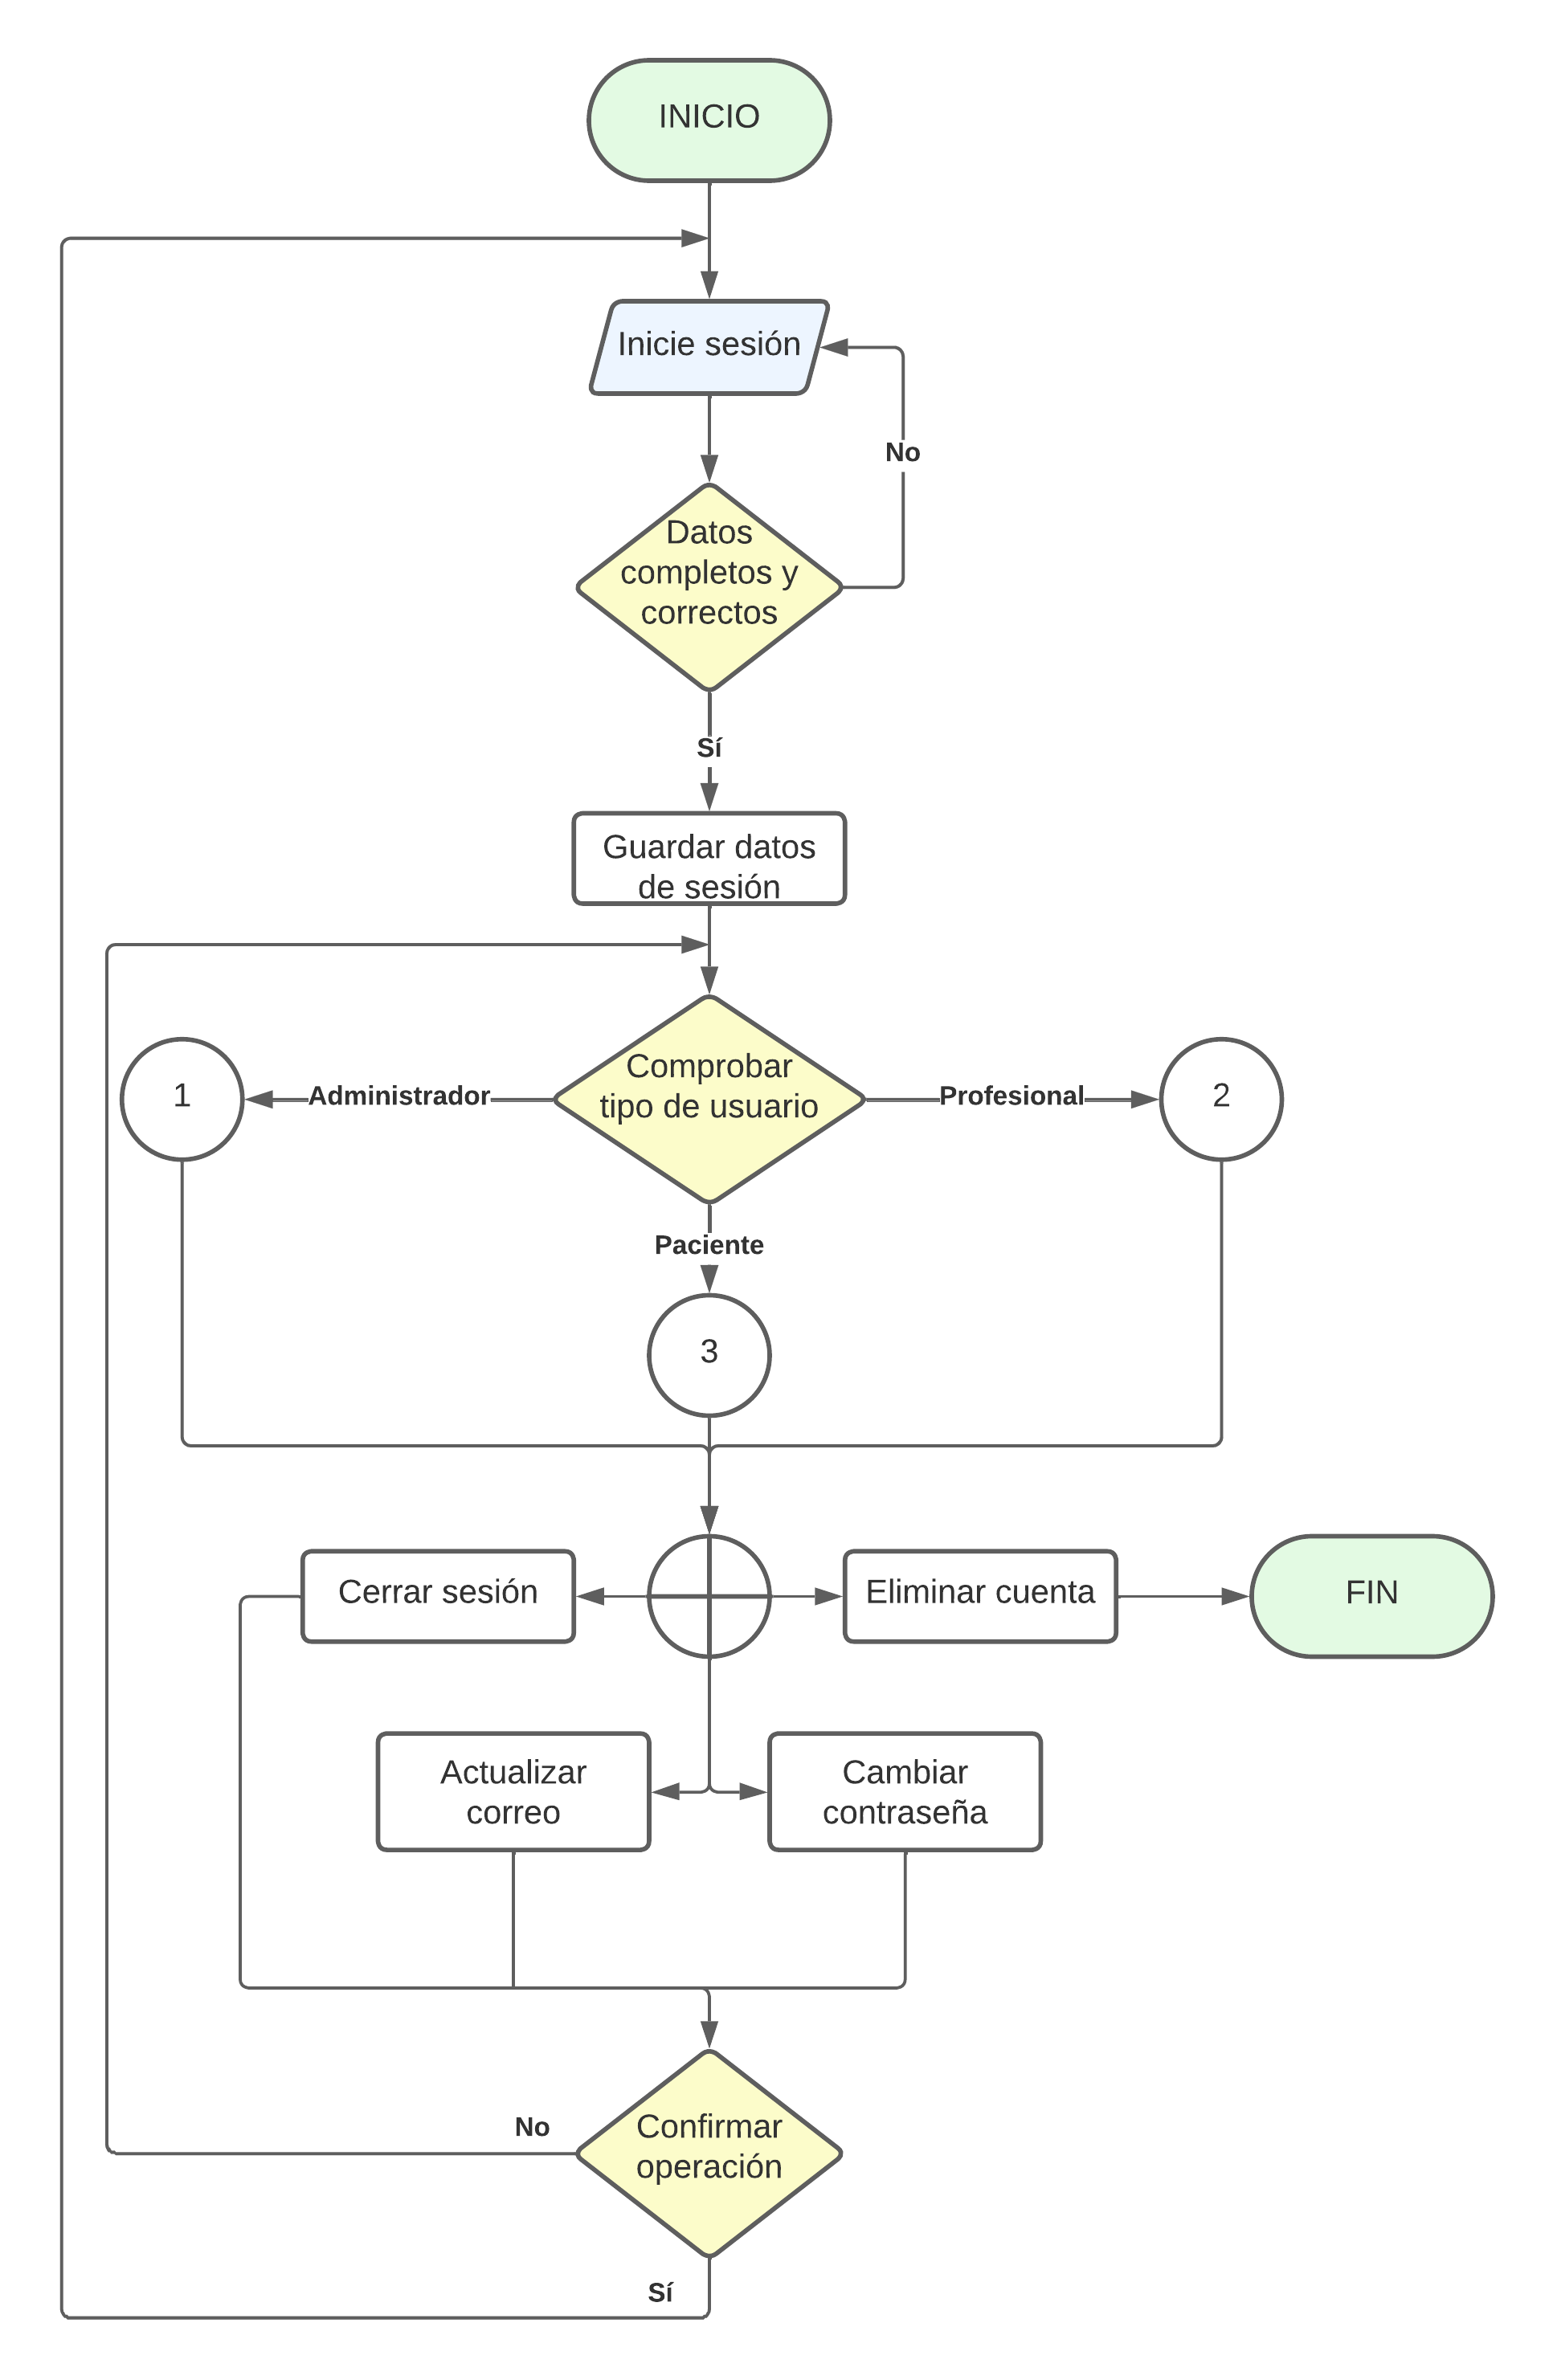
\includegraphics[width=1\textwidth]{img/E2_DiseñoArquitectonico/0_InicioFin.png}
    \caption{Diagrama de flujo - Inicio y fin de sesión.}
    \label{fig:0_InicioFin}
\end{figure}

\begin{figure}[h]
    \centering
    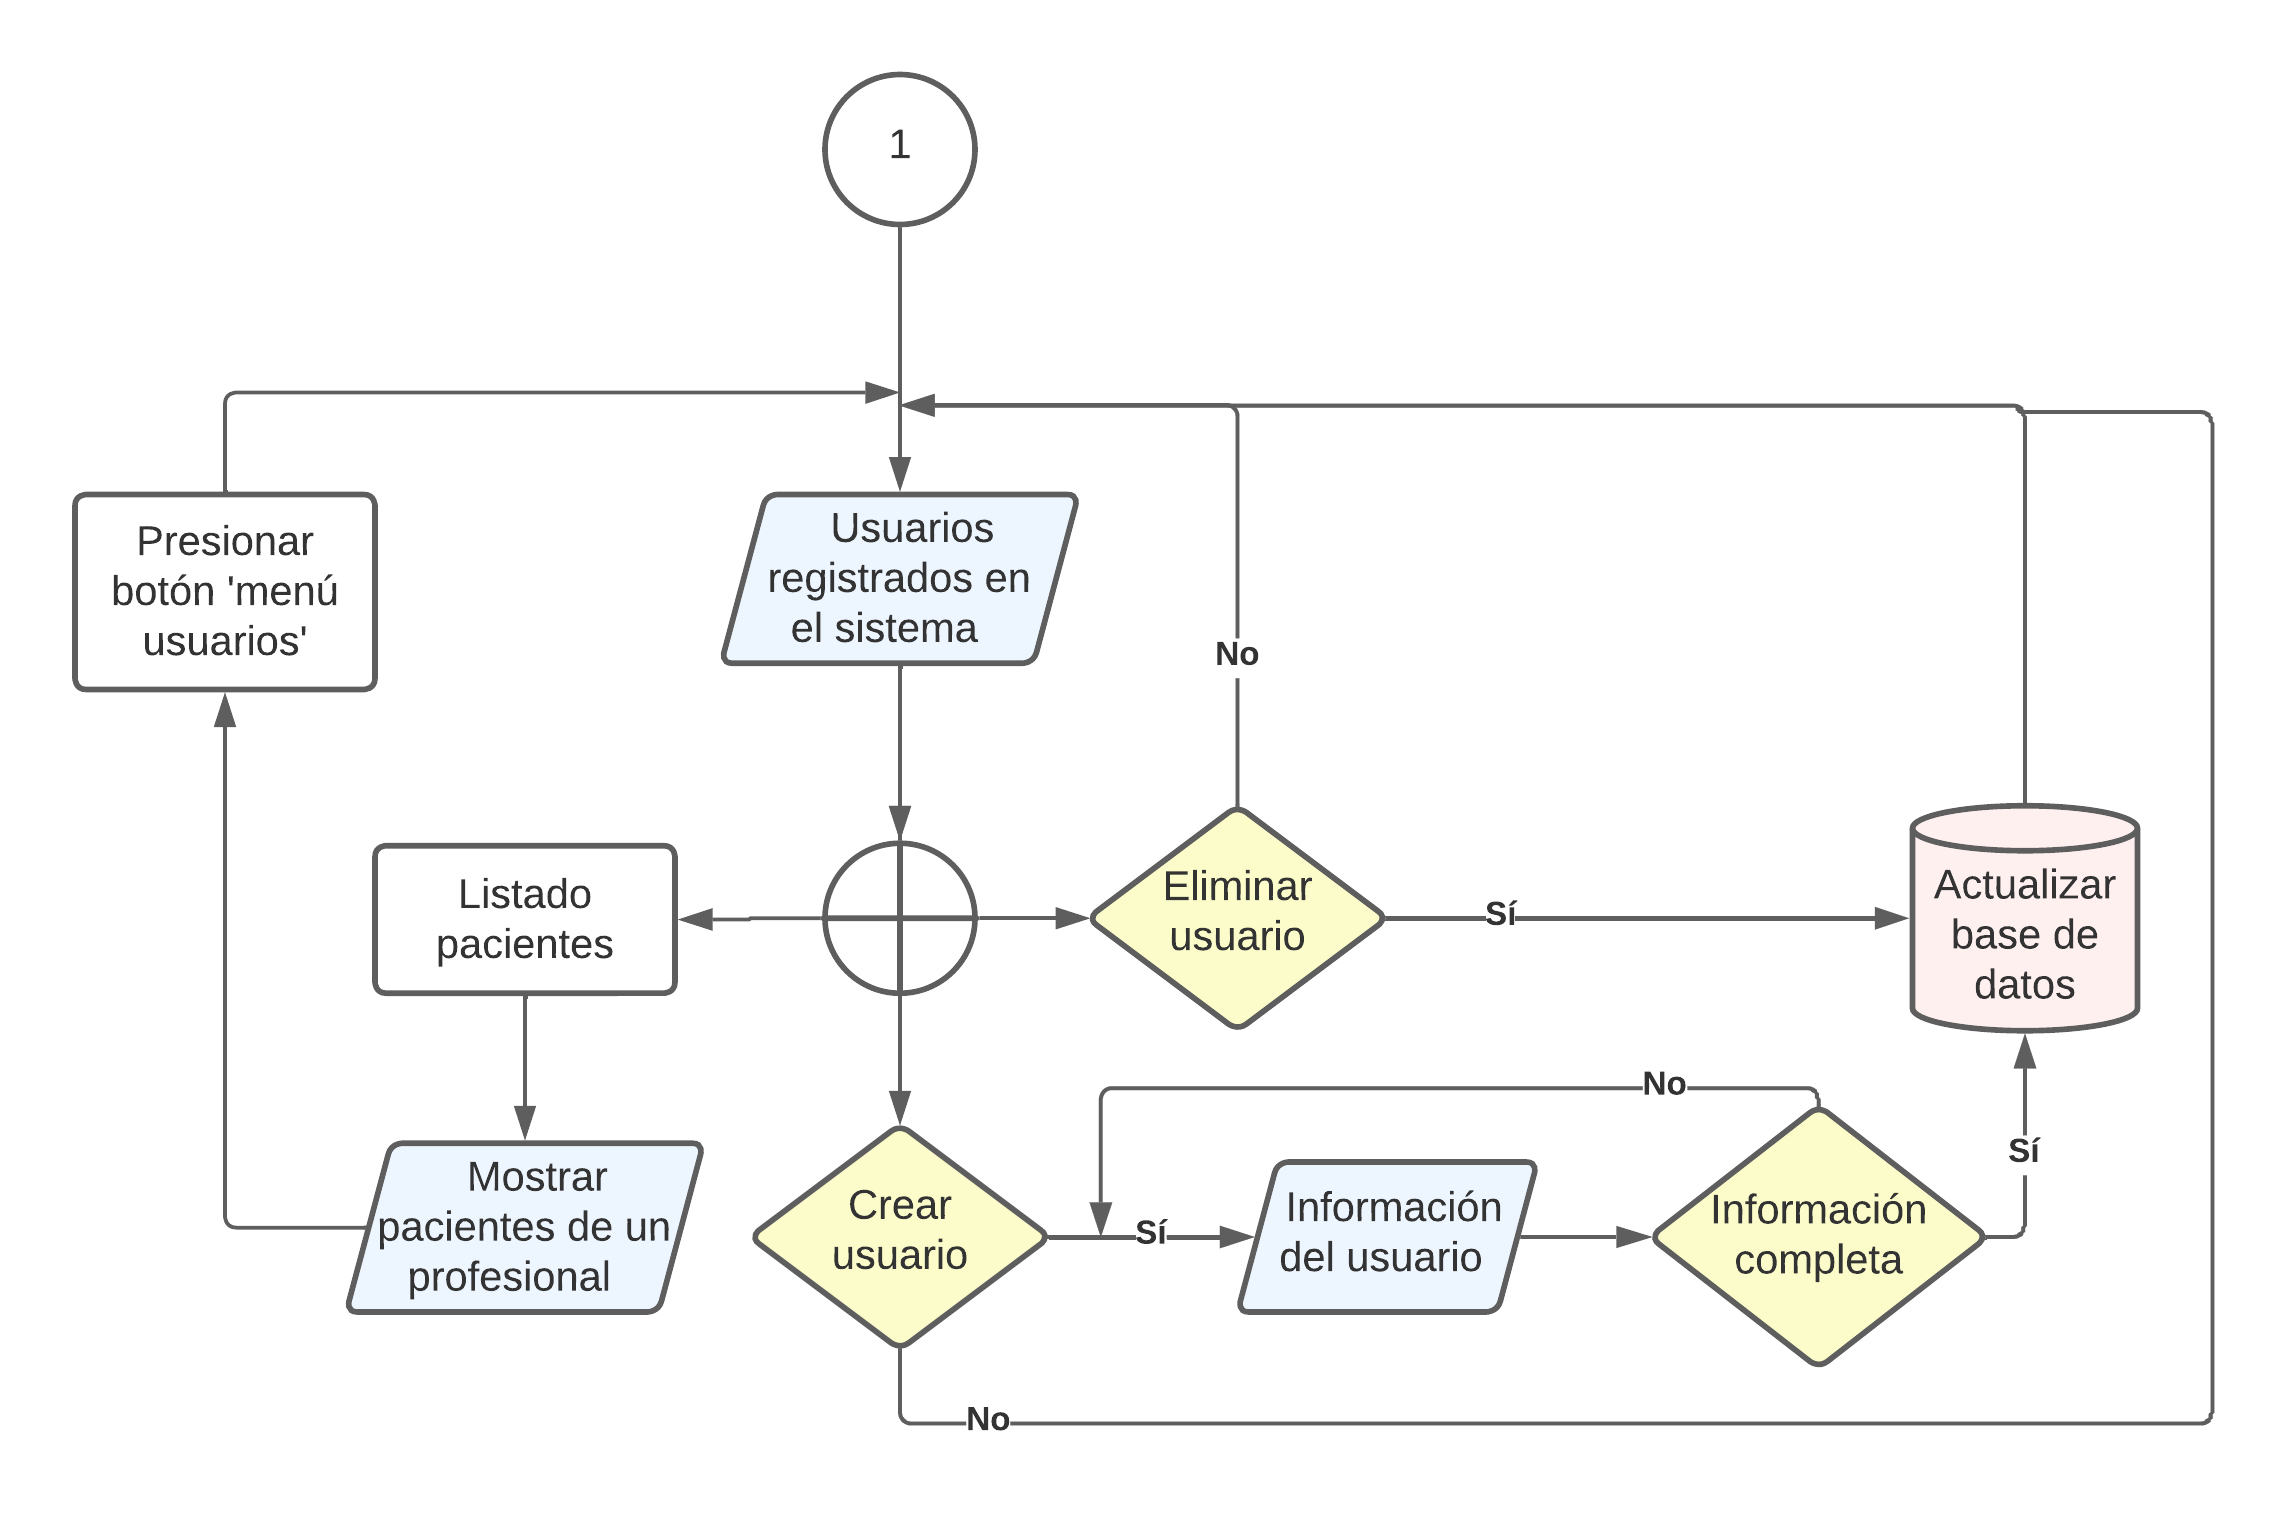
\includegraphics[width=1\textwidth]{img/E2_DiseñoArquitectonico/1_Admin.png}
    \caption{Diagrama de flujo. Usuario administrador.}
    \label{fig:1_Admin}
\end{figure}

\begin{figure}[h]
    \centering
    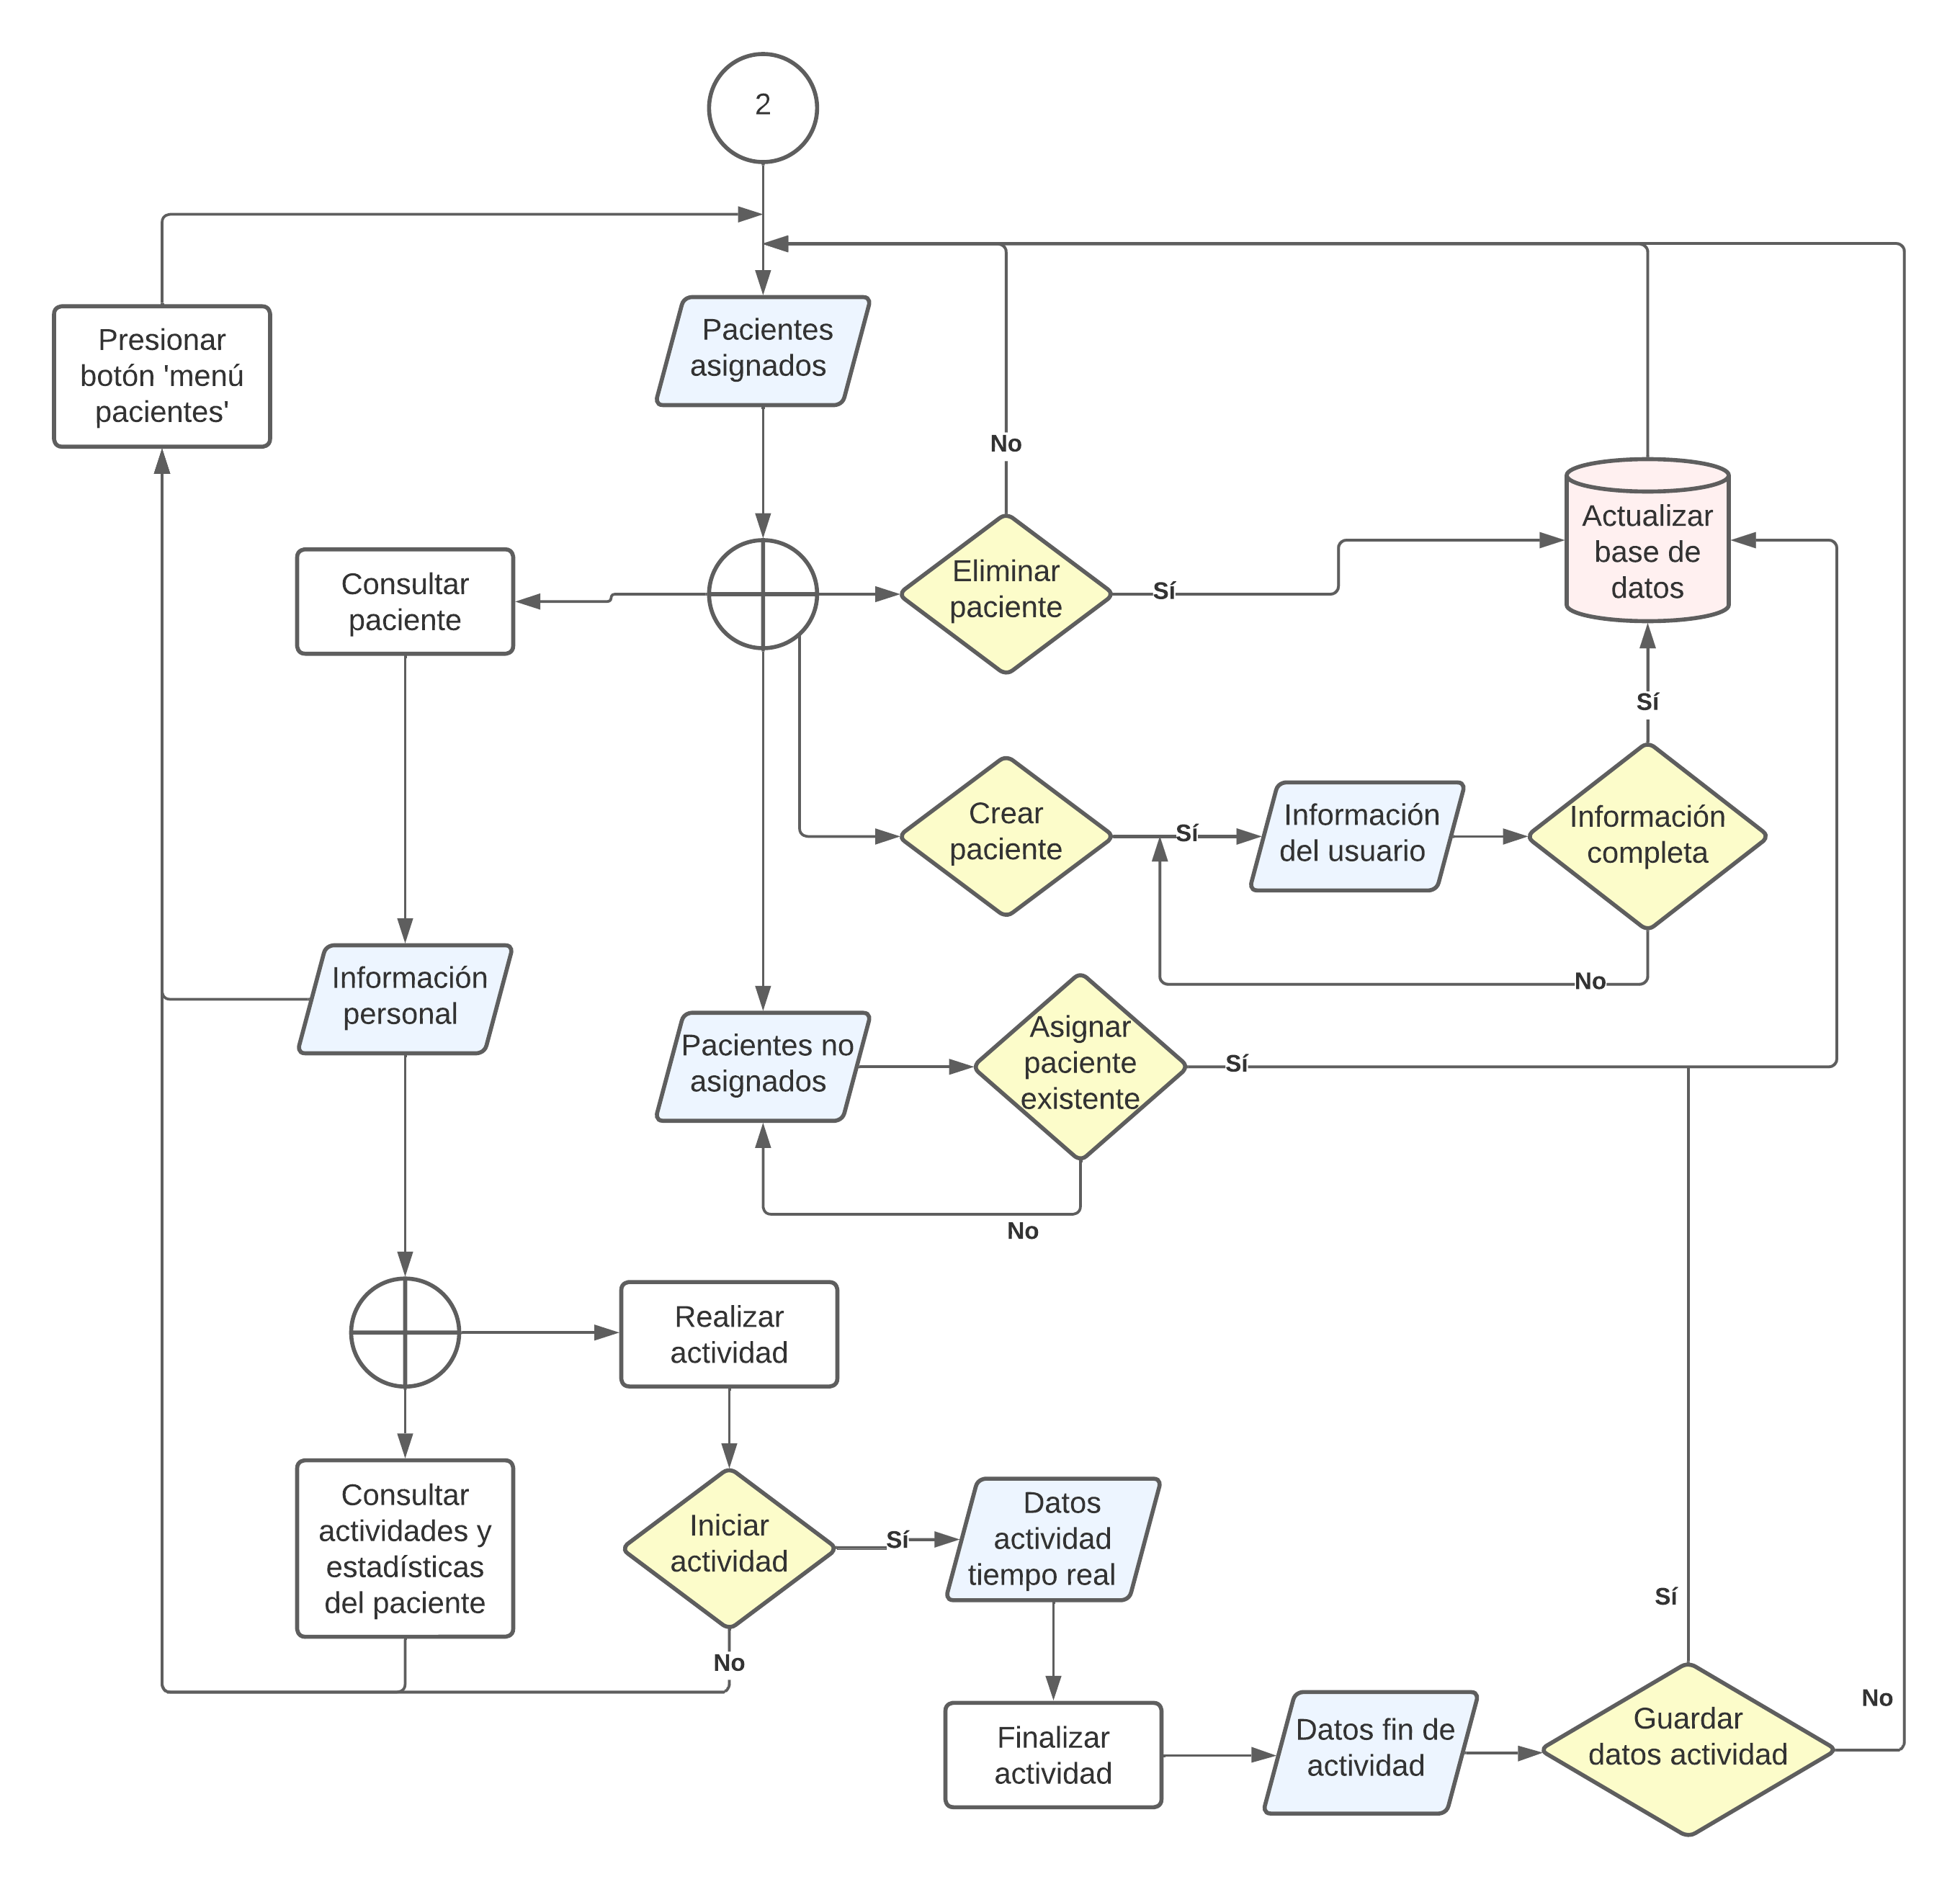
\includegraphics[width=1\textwidth]{img/E2_DiseñoArquitectonico/2_Profesional.png}
    \caption{Diagrama de flujo. Usuario profesional.}
    \label{fig:2_Profesional}
\end{figure}

\begin{figure}[h]
    \centering
    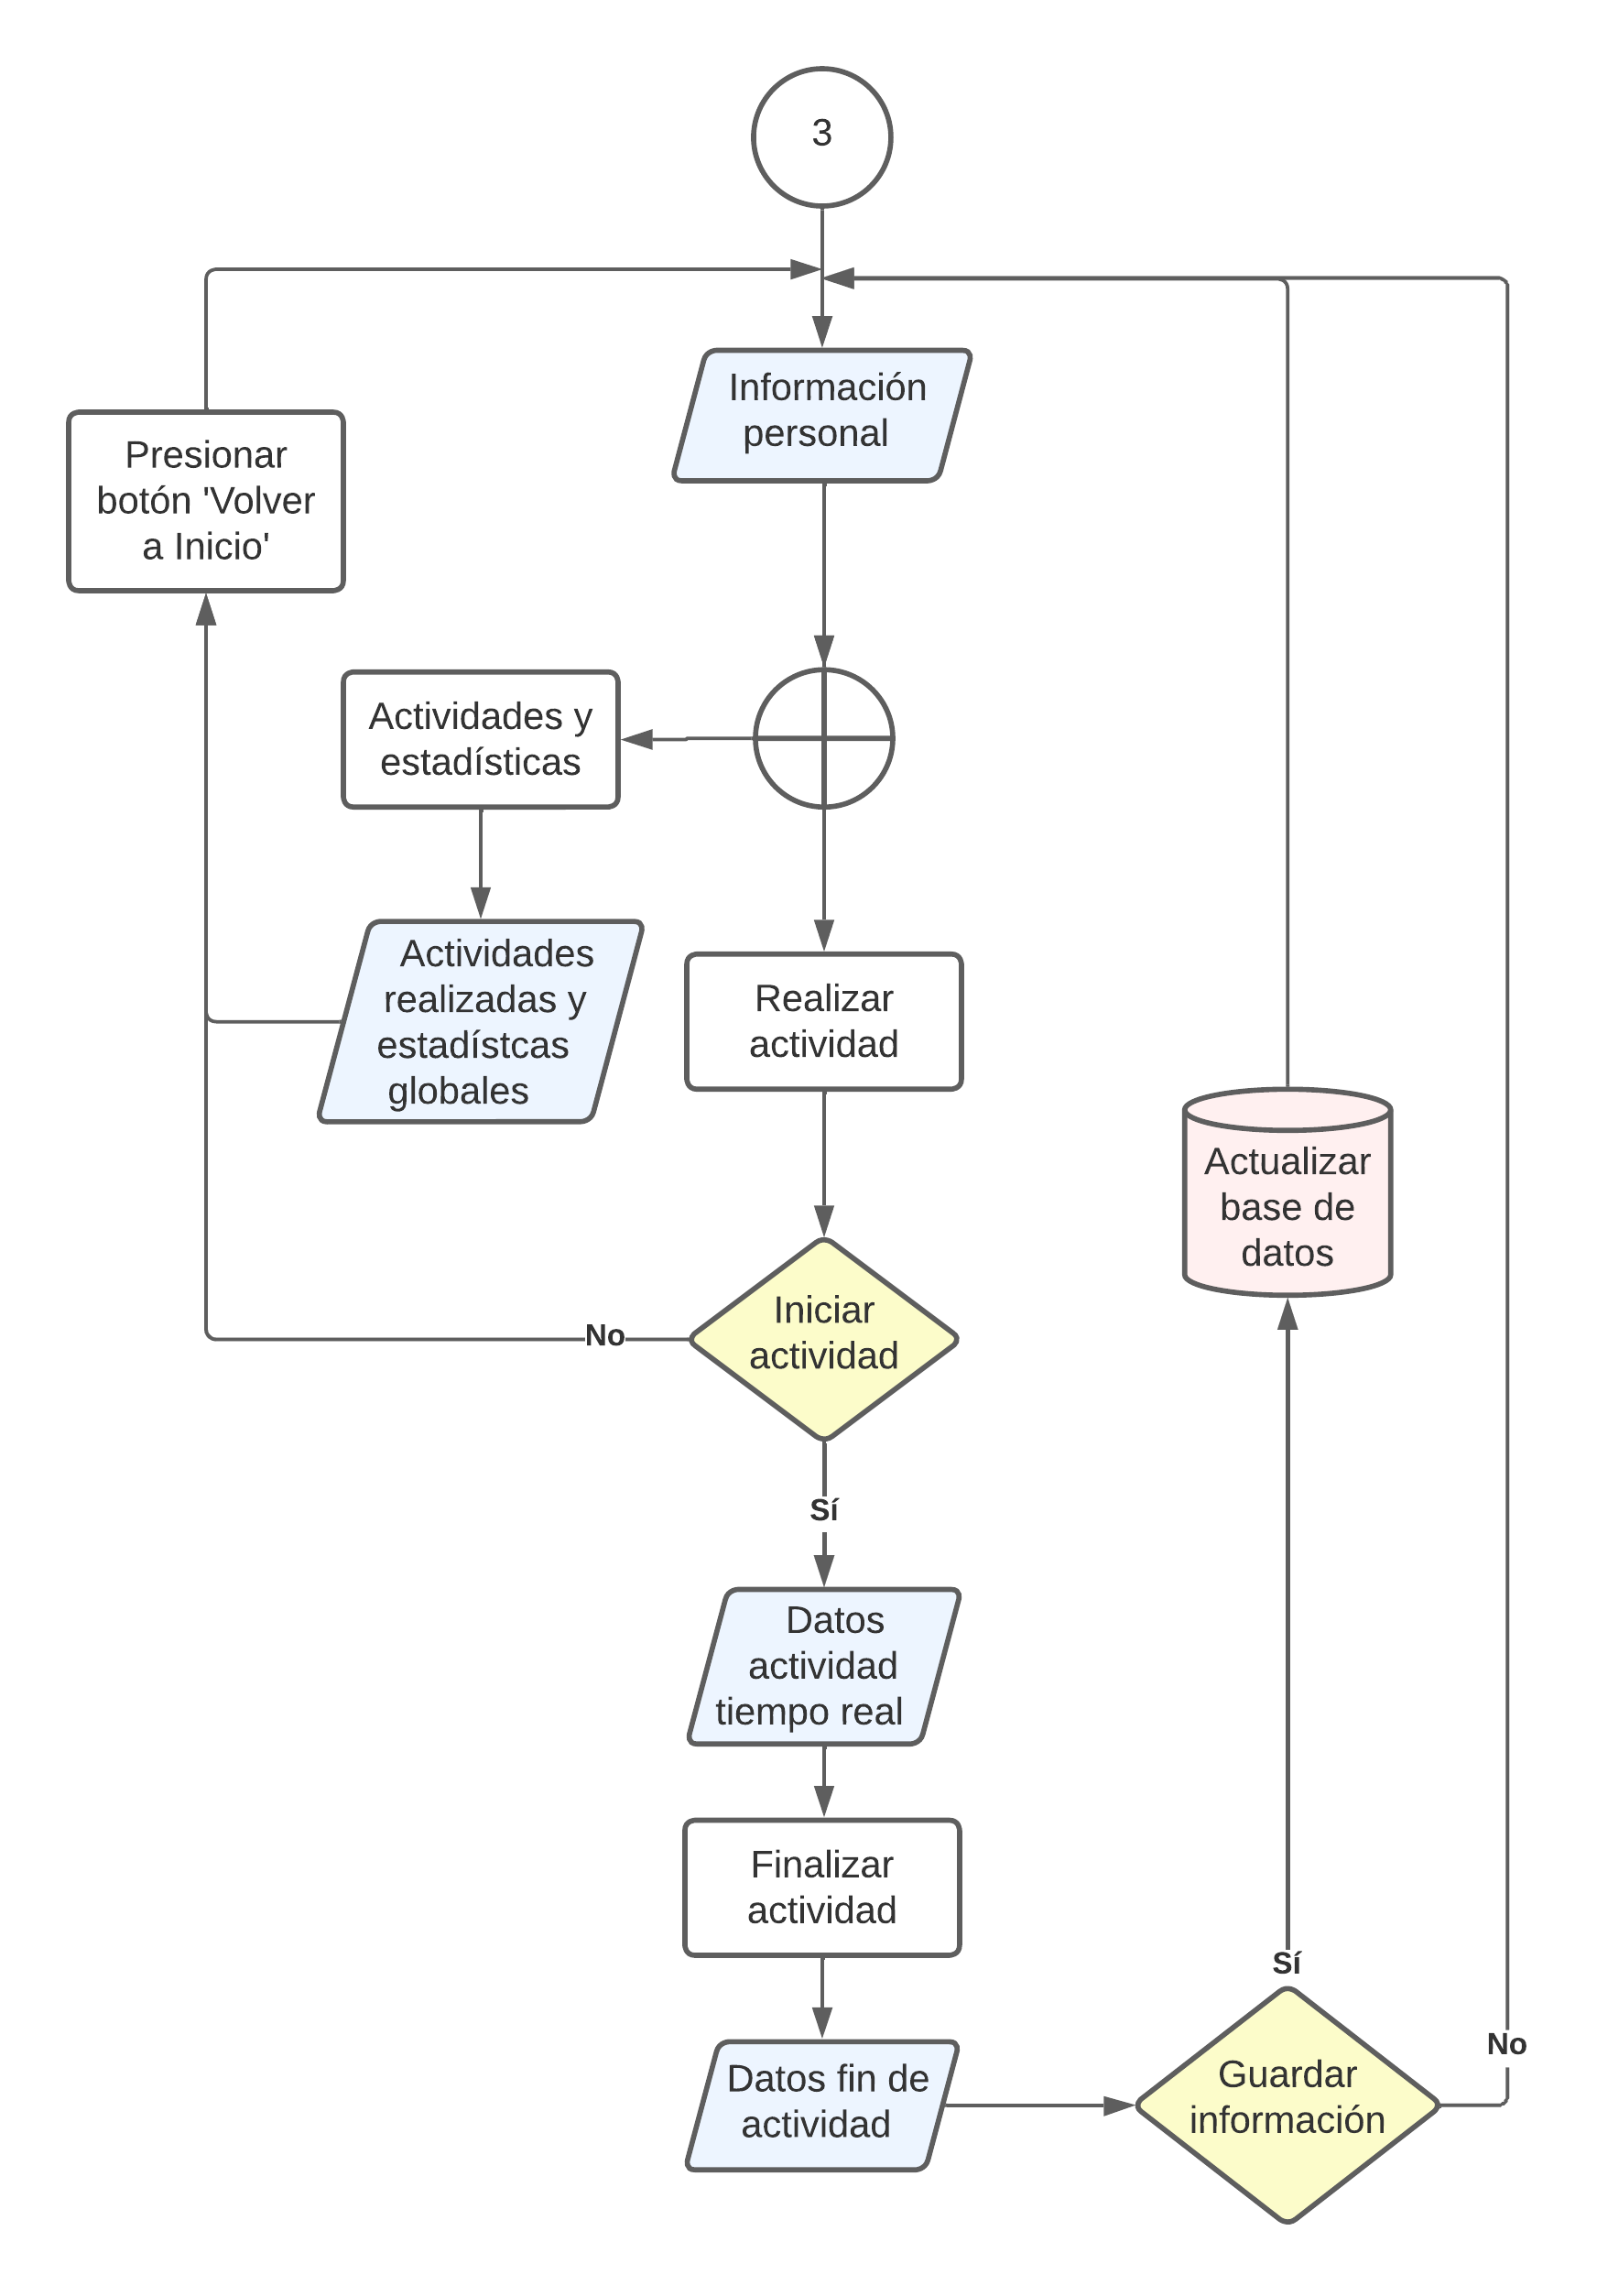
\includegraphics[width=1\textwidth]{img/E2_DiseñoArquitectonico/3_Paciente.png}
    \caption{Diagrama de flujo. Usuario paciente.}
    \label{fig:3_Paciente}
\end{figure}


En relación con el diseño de la interfaz de usuario, llevado a cabo mediante los wireframes que se presentan y describen en el \textit{Anexo F.3}, este se asocia principalmente con el desarrollo. Sin embargo, cabe destacar su alineación con la arquitectura web al establecer las pautas para la presentación de los elementos visuales.

\apendice{Especificación de Requisitos}

Si procede.

\section{Descripción requisitos funcionales}

\begin{itemize}
    \item \textbf{RF-01 Iniciar sesión}: Todos los usuarios deben introducir de forma obligatoria su correo electrónico, tipo de usuario y contraseña para poder acceder a la página web.
    \item \textbf{RF-02 Consultar pacientes y usuarios}: Otorgar acceso a la lista completa de usuarios o pacientes, según los permisos asignados al usuario, y permitir la realización de búsquedas específicas dentro de ella.
    \item \textbf{RF-03 Gestionar pacientes y usuarios}: Permitir la creación y eliminación de cuentas, así como la modificación de los datos almacenados en las cuentas de pacientes y médicos. La capacidad para realizar estas acciones depende del nivel de acceso que el usuario tenga en el sistema web.
    \item \textbf{RF-04 Realizar actividad}: Ofrece las opciones de iniciar y finalizar actividades, así como la opción de guardar o descartar estas mismas. Existirá la posibilidad de realización de actividades sin que exista conexión entre el dispositivo físico y la página web, el denominado "modo offline".
    \item \textbf{RF-05 Mostrar actividades}: Presenta al usuario las actividades realizadas por el paciente, ya sea a través de un calendario de actividades o una lista con aquellas que cumplen unos criterios establecidos por el propio usuario.
    \item \textbf{RF-06 Consultar estadísticas}: Visualización de los datos relacionados con las actividades realizadas por el paciente, ya sea de una actividad en concreto o de todas en conjunto.
    \item \textbf{RF-07 Gestionar cuenta}: Facilitar a los usuarios las tareas de cambio de contraseña y actualización del correo eléctrónico vinculado a su cuenta.
    \item \textbf{RF-08 Cerrar sesión}: Todos los usuarios tendrán la opción de cerrar sesión desde el menú de inicio. Para prevenir cierres accidentales, se solicitará una confirmación de la acción antes de que esta se complete.
\end{itemize}


\section{Diagrama de casos de uso}

\section{Explicación casos de uso.}

Se puede describir mediante el uso de tablas o mediante lenguaje natural.    

Una muestra de cómo podría ser una tabla de casos de uso:

% Caso de Uso 1 -> Consultar Experimentos.
\begin{table}[p]
	\centering
	\begin{tabularx}{\linewidth}{ p{0.21\columnwidth} p{0.71\columnwidth} }
		\toprule
		\textbf{CU-1}    & \textbf{Ejemplo de caso de uso}\\
		\toprule
		\textbf{Versión}              & 1.0    \\
		\textbf{Autor}                & Alumno \\
		\textbf{Requisitos asociados} & RF-xx, RF-xx \\
		\textbf{Descripción}          & La descripción del CU \\
		\textbf{Precondición}         & Precondiciones (podría haber más de una) \\
		\textbf{Acciones}             &
		\begin{enumerate}
			\def\labelenumi{\arabic{enumi}.}
			\tightlist
			\item Pasos del CU
			\item Pasos del CU (añadir tantos como sean necesarios)
		\end{enumerate}\\
		\textbf{Postcondición}        & Postcondiciones (podría haber más de una) \\
		\textbf{Excepciones}          & Excepciones \\
		\textbf{Importancia}          & Alta o Media o Baja... \\
		\bottomrule
	\end{tabularx}
	\caption{CU-1 Nombre del caso de uso.}
\end{table}

\section{Prototipos de interfaz o interacción con el proyecto.}



\apendice{Estudio experimental}

\section{Detalle de resultados.}

Este anexo presenta la encuesta SUS y los resultados obtenidos habiendo sido completada por una persona ajena al proyecto después de su primera experiencia usando el sistema.

Los 10 ítems de la encuesta se responden mediante una escala Likert con opciones de 1 a 5, donde 1 significa ``Totalmente en desacuerdo" y 5 ``Totalmente de acuerdo". Los resultados están contenidos en las Figuras \ref{fig:sus1}, \ref{fig:sus2}, \ref{fig:sus3} y \ref{fig:sus4}.

\begin{figure}[h]
    \centering
    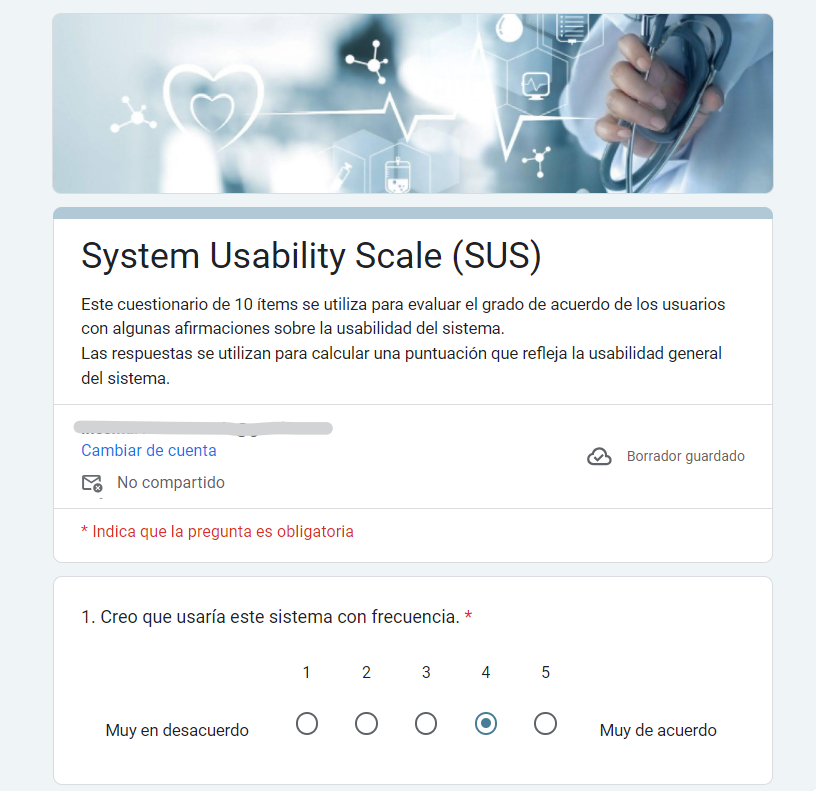
\includegraphics[width=1\textwidth]{img/G1_Resultados/sus1.png}
    \caption{Cuestionario SUS. Parte 1.}
    \label{fig:sus1}
\end{figure}

\begin{figure}[h]
    \centering
    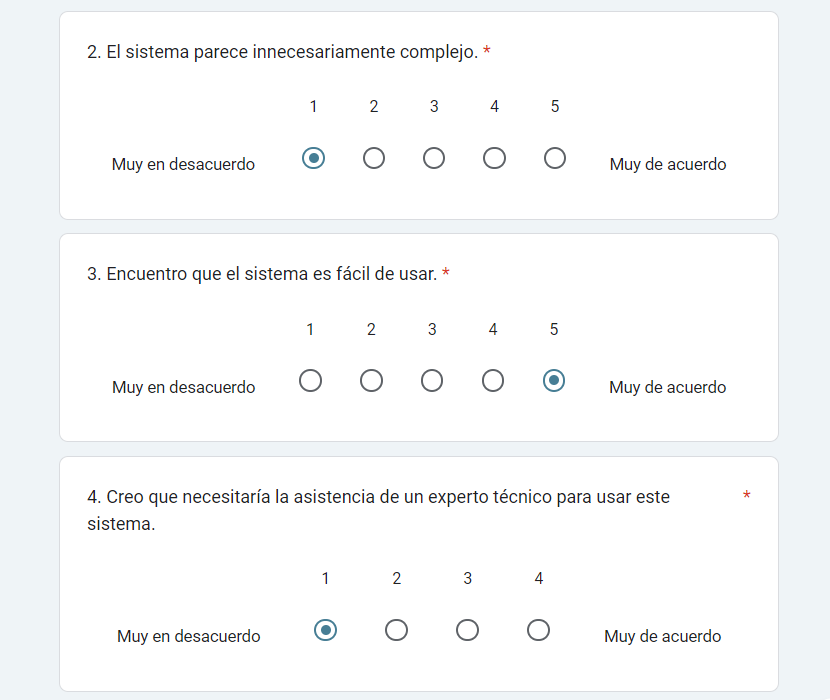
\includegraphics[width=1\textwidth]{img/G1_Resultados/sus2.png}
    \caption{Cuestionario SUS. Parte 2.}
    \label{fig:sus2}
\end{figure}

\begin{figure}[h]
    \centering
    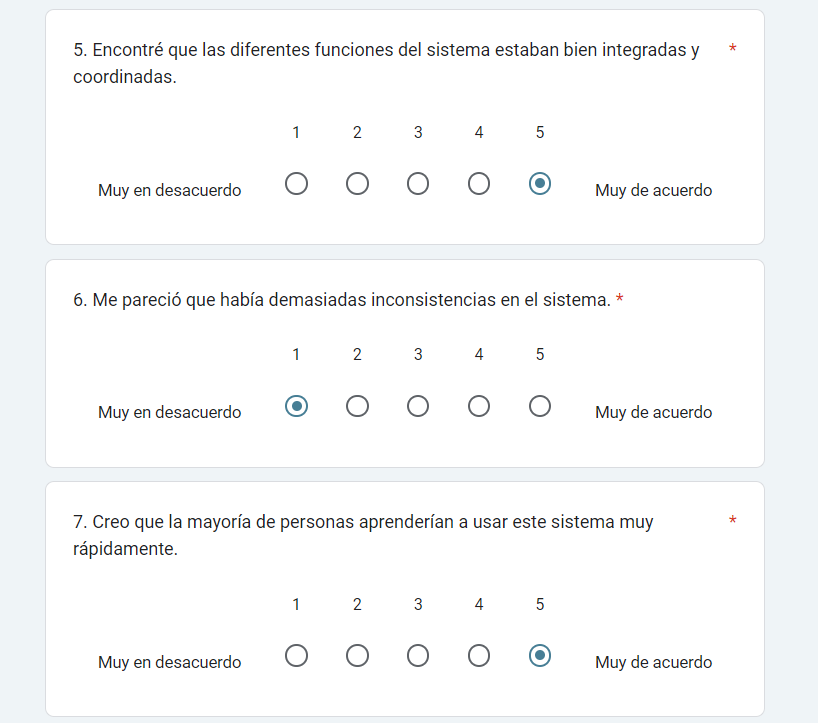
\includegraphics[width=1\textwidth]{img/G1_Resultados/sus3.png}
    \caption{Cuestionario SUS. Parte 3.}
    \label{fig:sus3}
\end{figure}

\begin{figure}[h]
    \centering
    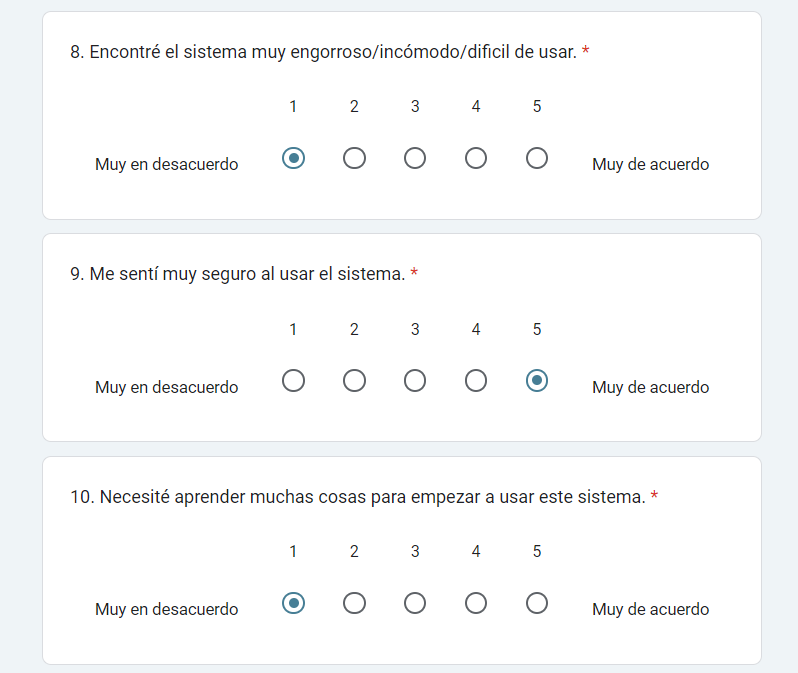
\includegraphics[width=1\textwidth]{img/G1_Resultados/sus4.png}
    \caption{Cuestionario SUS. Parte 4.}
    \label{fig:sus4}
\end{figure}

Para calcular la puntuación SUS, que pretende proporcionar un resultado objetivo sobre la usabilidad del sistema, se deben seguir los pasos descritos a continuación \cite{SUS}.
\begin{itemize}
    \item Suma de la puntuación de cada ítem (varía de 0 a 4) siguiendo las siguientes reglas para obtenerla:
    \begin{itemize}
        \item Ítems 1, 3, 5, 7 y 9, la puntuación es la posición en la escala menos 1.
        \item Ítems 2, 4, 6, 8 y 10, la puntuación es 5 menos la posición en la escala.
    \end{itemize}
    \item Multiplicar la suma de puntuaciones por 2.5.
\end{itemize}

En este caso se obtiene un \\SUS SCORE = ((3+4+4+4+4) + (4+4+4+4+4)) x 2.5 = 97.5 /100, \\resultado que supera ampliamente el punto de referencia (68) necesario para considerar que la web cumple de forma adecuada con su propósito.




\apendice{Anexo de sostenibilización curricular}

En el desarrollo de este Trabajo de Fin de Grado (TFG) he tenido la oportunidad de aplicar los principios de sostenibilidad adquiridos durante mi formación académica, profundizando en su comprensión más allá del ámbito teórico. Esta expereiencia me ha permitido entender el impacto y los riesgos que la actividad profesional de un ingeniero de la salud puede tener sobre la sociedad y el medio ambiente. 

A continuación, se describe cómo el proyecto respeta y se adhiere a los principios éticos de justicia social y calidad ambiental.

\begin{itemize}
    \item \textbf{Respeto a los derechos humanos y derechos fundamentales}.\\
    El enfoque del proyecto respeta los derechos humanos y fundamentales, particularmente el derecho a la salud y a gozar de los beneficios derivados del progreso científico. El uso de tecnología de bajo coste y la decisión de emplear hardware y software libre promueven la igualdad de todos los individuos para el acceso a la solución tecnológica obtenida.
    
    \item \textbf{Respeto a la igualdad de género, no discriminación y principios de accesibilidad universal}.\\
    El diseño sencillo e inclusivo de la interfaz de la página web garantiza la accesibilidad a todos los usuarios, independientemente de su género, edad, raza, capacidades físicas y habilidades tecnológicas. Las características del sistema lo convierten en un recurso valioso y accesible para cualquier paciente de Párkinson, contribuyendo a la inclusión. Otro aspecto que promueve la igualdad de acceso es la elección de software y hardware libre en el desarrollo del proyecto.
    
    \item \textbf{Tratamiento de la sostenibilidad y el cambio climático}.\\
    Consciente del impacto ambiental de la tecnología, en el desarrollo se ha querido reducir la huella ecológica en la medida de lo posible. Estas consideraciones condujeron a la elección de una batería recargable y materiales con una larga vida útil.
\end{itemize}

Este anexo, y el proyecto en su conjunto, reflejan mi compromiso con una evolución tecnológica innovadora que responde a las necesidades sociales, de acuerdo con la protección de los derechos humanos y atendiendo a la actual situación de crisis climática.





\bibliographystyle{apalike}
\bibliography{bibliografiaAnexos}

\end{document}
